\section{Automated conformance testing for IoT applications}
\label{sec:smartcity_testing}
In the upcoming decades, people living in the cities are going to be surrounded by billions of IoT devices that will interoperate and collaborate with each other to deliver personalized and autonomic services. As a result, citizens could be the first to benefit from the technologies in the cities. However, relying on these machines to make decisions could bring profound problems if cities cannot ensure the reliability of those IoT services~\cite{loper2017machine}. For instance, currently, many IoT devices are being deployed and operated for supporting various IoT services such as smart vehicles, surveillance cameras, smart buildings.

However, if IoT devices do not assure their reliability, connecting all the systems to the Internet can cause severe problems in the cities~\cite{kaiser2019standards}. Therefore, to avoid the problems caused by dysfunctional products or not working IoT services, it is necessary to test all the IoT platforms and devices before releasing them in smart cities. Furthermore, smart cities are operating IoT platforms and devices using various standards and protocols, which means that smart cities have to consider these environments as well. Based on the previous discussion, to realize and to assure the safety of smart city environments in the highest level, this section starts by introducing the adaptable IoT testing framework to support the IoT testing. In addition, to mitigate the testing error and to reduce the testing time, an automated IoT testing architecture and procedures are proposed.


\subsection{Analysis of the traditional IoT testing}
For the last two decades, the interoperability is the main hurdle of IoT proliferation and adoption~\cite{roman2013features, khan2012future, miorandi2012internet}, and to successfully adopt the IoT into the industry fields, it is imperative to overcome its fragmentation issue between IoT services~\cite{bandyopadhyay2011internet, song2014connecting}. Therefore, assuring the interoperability of IoT implements based on differing standards and protocols requires well known conformance and interoperability testing process in the software industry~\cite{vallejo2007state, seol2003fully, maag2008interoperability, hao2004integrated, schmidt2007ims}. In this regard, IoT conformance testing is becoming one of the most important parts of IoT technologies~\cite{ahmed2019aspects, sand2015iot}. Conformance testing is considered to be an essential element of the IoT testing to provide a reasonable degree of gurantee and it is used to check systems or devices that are well developed against the standards developed by telecommunication organizations~\cite{kone2000test, zhang2004ipv6, howden1980functional}. In addition, in the paper~\cite{kim2017towards}, International Telecommunication Union (ITU) has been recognizing that interoperability testing is highly important to ensure that independent implementation based on the same standard are interoperable. With the importance of IoT testing as described, in the subsequent subsection, this dissertation goes deeply to describe the conformance and interoperability testing.

\subsubsection{Conformance and Interoperability Testing}
Conformance testing is one of the testing approaches where a system is tested against its standard specification~\cite{rayner1987osi,krichen2009conformance,krichen2004black}. The aim of conformance testing is to improve the confidence of the implemented system's probability that it follows the same standards. It is possible to find the expected or unexpected (invalid) behavior of the specific protocols but conformance testing does not cover all aspects because it only tests the systems against specific scopes or requirements specified in testing specifications. In addition, it does not actually test how well the system works with other systems. Conformance testing specifications for Global System for Mobile Communications (GSM), Universal Mobile Telecommunication System (UMTS) and Voice over Internet Protocol (VoIP) was developed by European Telecommunications Standards Institute (ETSI) and test specifications were developed according to the well-proven ISO/IEC 9646 conformance testing methodology~\cite{moseley2003experience}. The conformance testing specifications are also referred to the major elements of ISO/IEC, and the widely used procedures are described in Fig.~\ref{fig:procedures_of_the_conformance_testing}~\cite{moseley2003experience}. In addition, the main components that make up the procedures are as follows.

\begin{figure}[tb!]
\centering
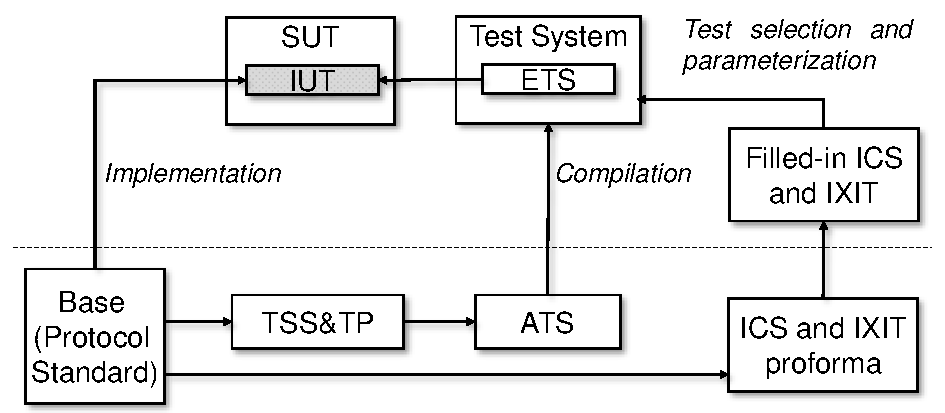
\includegraphics[width=\textwidth]{figures/fig_conformance_testing_procedures.pdf}
\caption{Procedures of the ETSI Conformance Testing}
\label{fig:procedures_of_the_conformance_testing}
\end{figure}

\begin{itemize}
  \item \textbf{The Test Suite Structure and Test Purpose (TSS) \& Test Purpose (TP):} These are derived from the relevant base standard. They provide an easy-to-read and informal description of each test. In addition,  these concentrate on the meaning of the test rather than detailing how it may be achieved.
  
  \item \textbf{The Abstract Test Suite (ATS):} It is the entire collection of test cases. Each test case specifies the detailed coding of the test purposes written usually in a test specification language such as the standardized TTCN.

  \item \textbf{The Implementation Conformance Statement (ICS) \& The Implementation eXtra Information for Testing (IXIT): } These contain additional information (e.g., specific addresses, timer values etc.) necessary for testing.
  
  \item \textbf{The Executable Test Suite (ETS): } It can be quickly and easily implemented from the ATS using the TTCN compilers available on most modem test tool platforms (C++, Java etc.).
  
  \item \textbf{System Under Test (SUT) \& Implementation Under Test (IUT): } SUT is the real open system~\cite{2016etsitestingspec}, and inside there is IUT which is the implementation of applications, services or protocols.
\end{itemize}

\begin{figure}[H]			% Add figure one
	\centering
	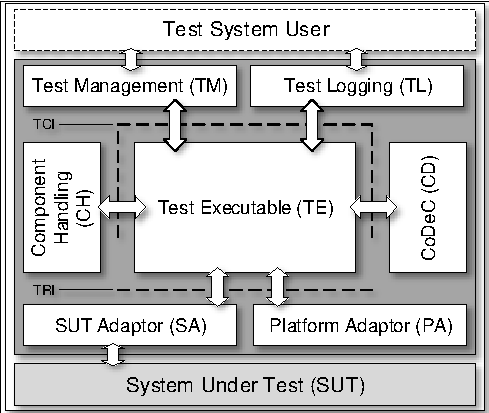
\includegraphics[width=10cm,height=9cm]{figures/fig_TTCN3_conceptual_testing_framework.pdf}
    \caption{TTCN-3 conceptual testing framework}
    \label{fig:ttcn-3_conceptual_testing_framework}
\end{figure}

Regarding the test cases described in ATS, TTCN-3 dedicated language for the protocol testing was developed and are being maintained by ETSI and also it is redesigned language based on tree and tabular combined notation (TTCN) standard (ITU-T Rec. X.292). TTCN-3 is an applicable language to the specification in terms of testing the reactive system and it is widely used in following areas such as protocol testing, service testing, module testing and Application Programming Interfaces (APIs) for the platform~\cite{grabowski2003introduction}.

TTCN-3 defines a independent standardized conceptual model against the SUT, processing platform, implement the language. The well-defined sets of operations of each entity and interfaces for providing communication, management, external data, and logging can be executed by implementing and interpreting to intermediate languages.
The general concept consists of the TTCN-3 based Testing System (TS) is shown in Fig.~\ref{fig:ttcn-3_conceptual_testing_framework}. The TTCN-3 test system performs conformance testing through interactions between entities that include specific functions and each independent entity has functionalities such as communication with the System Under Test (SUT), timer management, type handling, and external function call. In addition, there are interfaces called TTCN-3 Control Interface (TCI) and TTCN-3 Runtime Interface (TRI). Through the interactions between Test Executable (TE) which is responsible for the execution of the TTCN-3 module and two interfaces including TCI, TRI, actual TTCN-3 modules are executed. Following five entities make up TTCN-3 conceptual testing system and detailed entities functionalities are as follows~\cite{willcock2005introduction}. First, entities that communicate with TE by using TCI interface are as follows.

\begin{itemize}
  \item \textbf{Test Management (TM):} TM entity acts as a managerial layer of a test system. On this entity, the test developer defines the arrangement of the test suite execution list. Through this layer, TTCN-3 provides support test campaigns creation, log format and handling customization. 
  
  \item \textbf{Component Handling (CH):} Since TE can work in either centralized way or decentralized way, the aim of CH is for synchronizing entities which could be placed on different nodes and for managing the interaction between them.
  
  \item \textbf{CoDec (CD):} Codec is designed for encoding/decoding outgoing and incoming message during bidirectional transmissions toward SUT. In order to communicate with SUT, TTCN-3 abstract data representation format has to be converted actual format required by standard-based IUT tested.
  
  \item \textbf {Test Logging (TL):} All log events generated by the testing system are handled. The testing system must provide a log system for debugging purposes.
\end{itemize}

The following types of entities communicate with the TRI interface:

\begin{itemize}
  \item \textbf{SUT Adapter (SA):} This is responsible for the actual communication with the  SUT. That is, messages are transmitted to the SUT according to a specific procedure. In addition, messages are transmitted by the SUT with the testing results. The main activity happened inside SA is a bidirectional transmission of messages and procedure toward SUT. SA usually has concurrent and synchronous characteristics as the result of its aim to be retriever and sender of messages and procedures. Therefore, there are individual thread performances to deal with incoming and outgoing data.
  \item \textbf{Platform Adapter (PA):} It is mainly characterized by the support of timer function and the external functions including communication functionalities, and the timer function is used to control the flow of TTCN-3 code by using time literally. In particular, the external function makes the TTCN-3 language even more powerful because it uses a library implemented in the native language such as C++ or Java, which makes it possible to use additional functions not supported by TTCN-3. 
\end{itemize}

Unlike the conformance testing that is usually testing the single systems or devices to check whether they are well following the standard, interoperability testing is based on the interaction of systems or devices. At this time, there is much literature regarding interoperability, but one book published by ETSI is describing the interoperability testing comprehensively, so the following descriptions are based on ~\cite{etsibookforinterop}. The trend of a global interconnection demonstrated by the huge growth in the IoT makes no longer a single standard body is leading entire technologies. Usually, complex products and system are based on multiple standards from multiple standard bodies such as ETSI, IEEE, ITU-T and those have different aspects and features to support the specific services. To conclude, it is important to reduce the ambiguities, errors, unclear requirements that could lead to non-interoperability. At present, there is no single and specific definition of interoperability testing but, according to the ETSI's interoperability definition, ``Interoperability can be considered to be the ability of two or more systems or components to exchange data and use information". Once a set of requirements of systems or devices using specific standard has been identified and defined, it is important to check if they provide interoperable solutions. Many issues can be identified and resolved through technical specifications, but only through interoperability events or actual tests,  interoperability can be ensured. For instance, ETSI complements support for other testing activities by integrating Plugtests™ into the standardization process. In this regard, the results of the Plugtests™ event provide valuable feedback to other international organizations and forums.

\begin{figure}[H]			% Add figure one
	\centering
	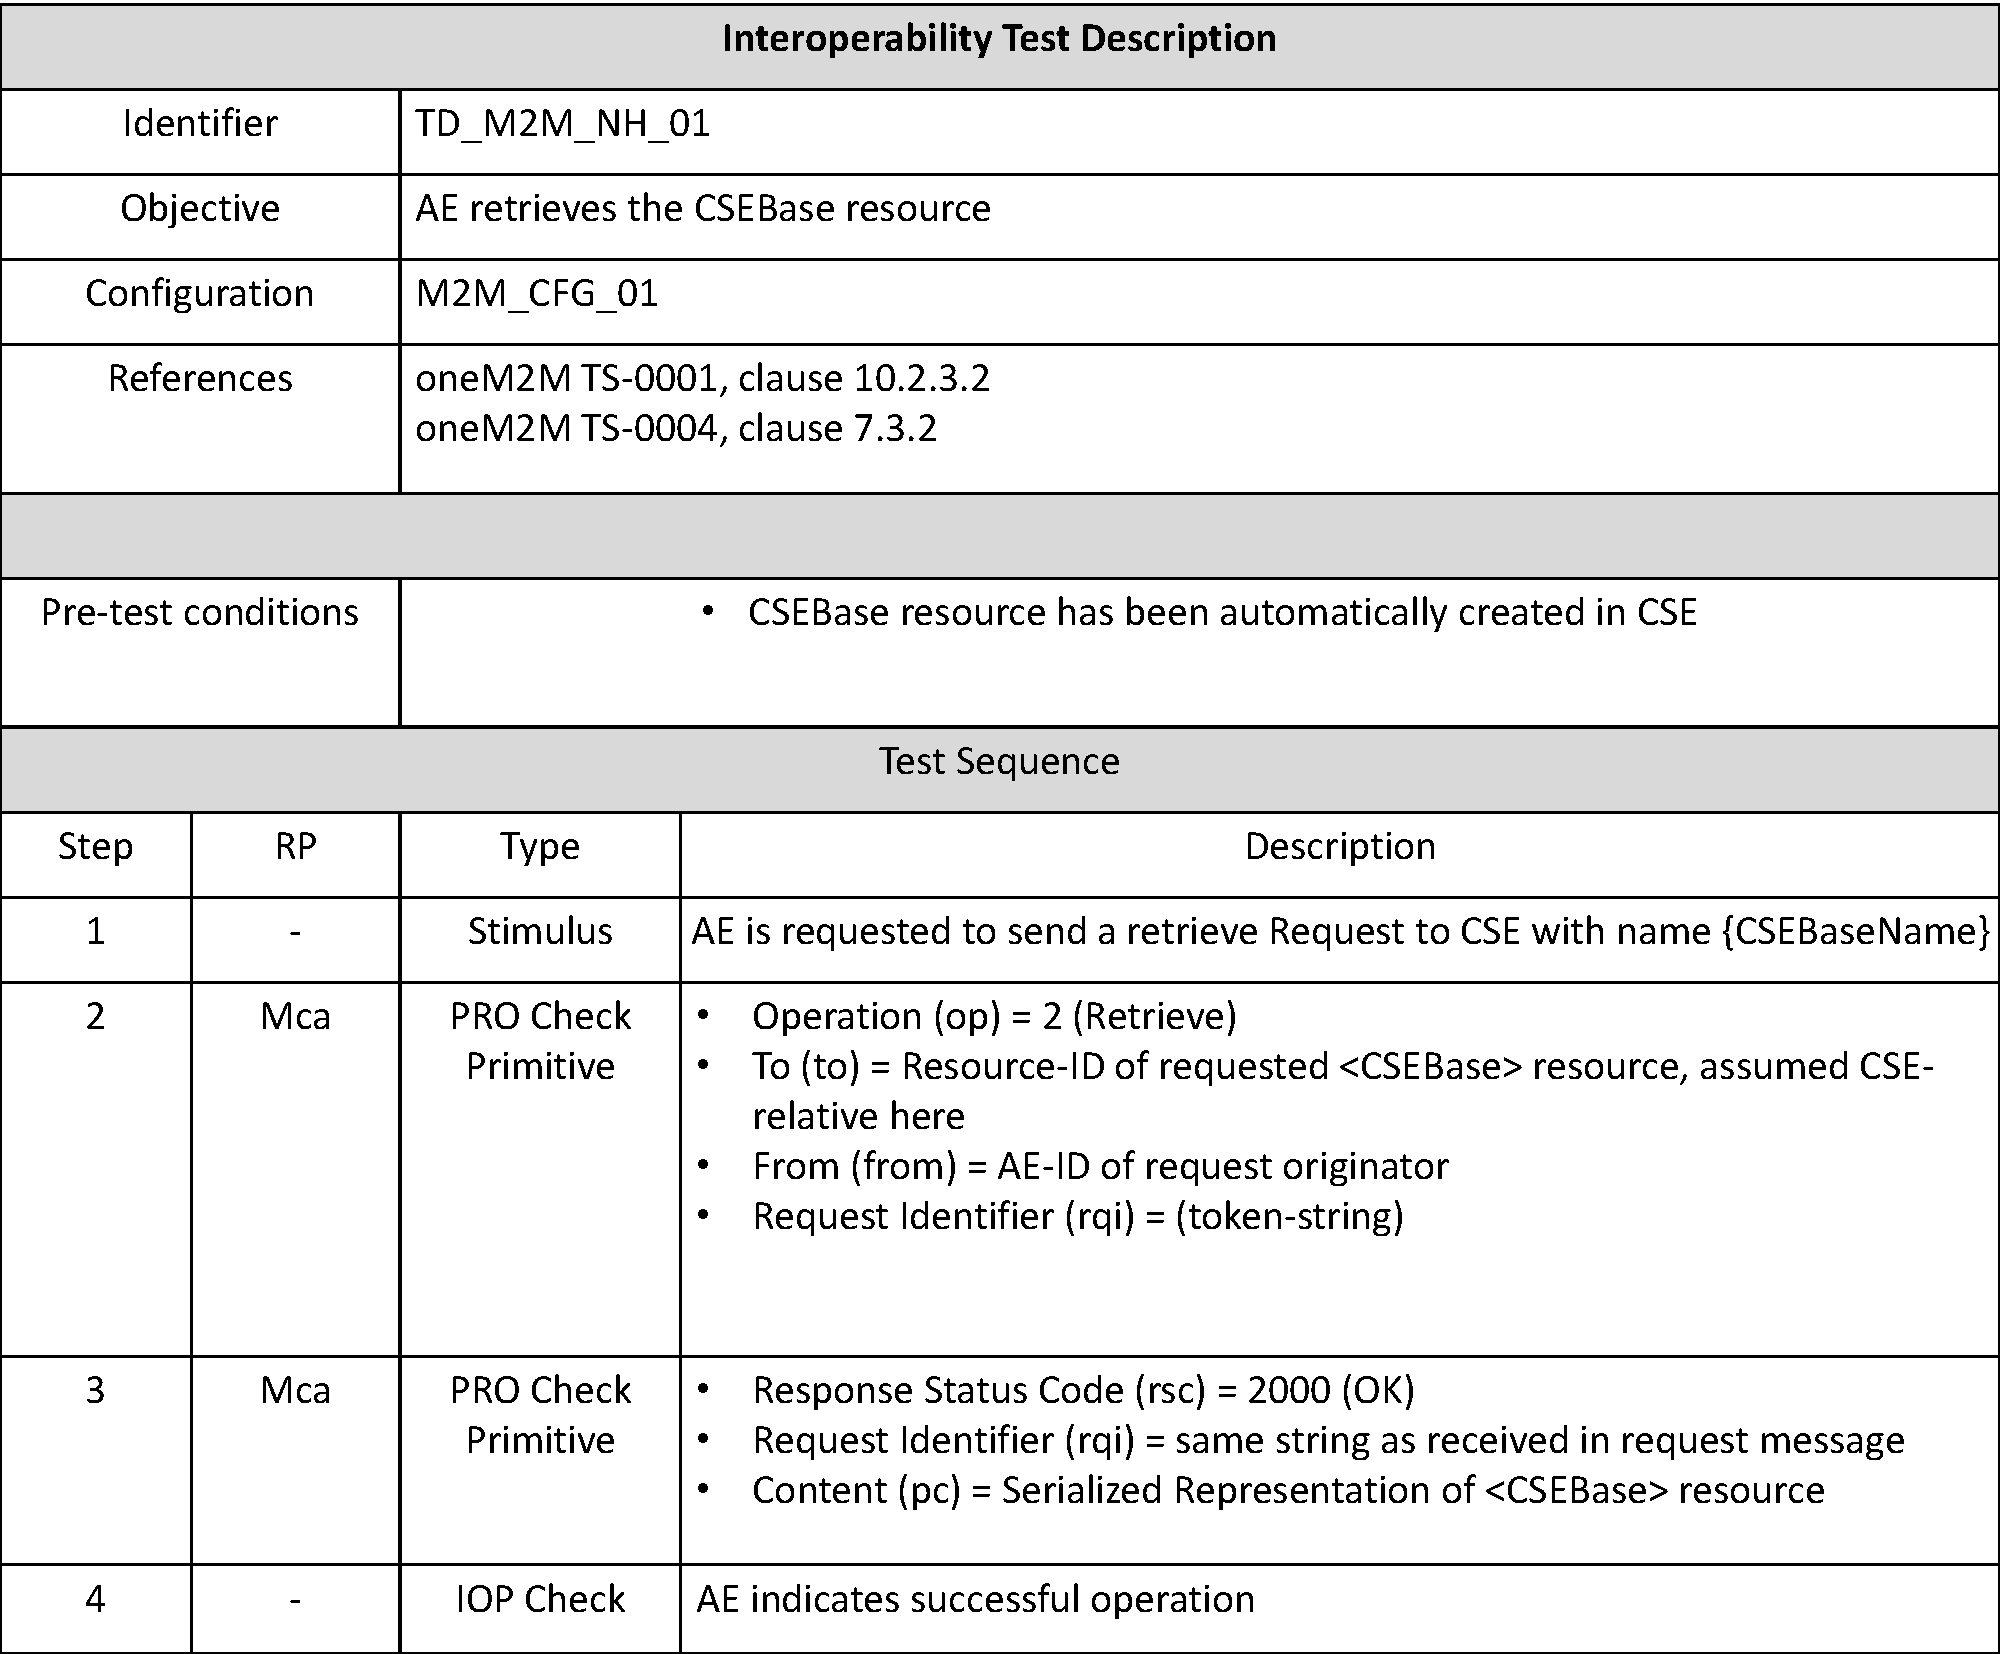
\includegraphics[width=\textwidth]{figures/fig_interoperablity_testing_description.pdf}
    \caption{oneM2M interoperability testing descriptor}
    \label{fig:interoperability_test_descriptor}
\end{figure}

Interoperability testing often involves activating and observing user functions, so it makes to specify test cases as a series of steps that human test drivers will perform. In some cases, it is not necessarily all, but it is useful to be able to specify some preconditions for the test. This often takes the form of instructions for configuring the network and equipment so that the testing objectives are fully met. The test steps themselves should be specified in a clear and unambiguous way, even though there are no unreasonable restrictions on how each step is performed. Clarity and accuracy are important to ensure that steps are performed accurately. The ``pass" determination always means that the connected device works correctly for certain tests, but it does not imply that the ``failure" determination does not. Interconnected network equipment plays an essential role in almost all interoperability testing, but is not usually included in the equipment under test. The ``failure" judgment can be caused by a network defect or unexpected behavior. Therefore, each ``failure" judgment must go through a thorough investigation. If possible, monitoring equipment should be used to determine the root cause before re-inspection (if the root cause is within the tested device) before verifying the judgment result as a real failure. Test steps and judgments should be specified at a level appropriate for the function to be tested. Based on these requirements, interoperabilty test description is being developed as described in Fig.~\ref{fig:interoperability_test_descriptor}~\cite{2018_ts_0013_interoperability}. 

\subsubsection{Related work of traditional IoT testing}
\label{sec:related_work}
\noindent
In~\cite{frameworkIoT2017}, it briefly explained the concept of a
testing framework for IoT by integrating the concept of simulation,
unit integration and end-to-end integration testing.
In addition,~\cite{ensuringCompliance2018} explored compliance
of IoT devices with privacy policy agreements and established models
regarding the privacy criteria to measure the degree of
compliance. However, those approaches have the disadvantages that both
testing systems and test experts must be physically located at the
same place to test their products.

Accordingly, the cloud-based testing system has been a great
alternative for dealing with the previous issue. The characteristics
of cloud computing can enhance service
delivery~\cite{testingInCloud2012}, production cost and time
reduction~\cite{taas2013} and responsiveness towards requirement  
changes. In this regard, cloud computing can be used as an IoT testing
platform remotely supporting IoT testing, logs and results views. The
F-Interop~\cite{fInteropImplementation2018}, a cloud-based
interoperability testing framework, 
provides a testing expert remote testing environment supporting a
variety of IoT standards and protocols and standards. However, it
heavily concentrates on the interoperability
aspect. ~\cite{IoTTestware2017} developed TTCN-3-based testing suites
called IoT-Testware to support the widely used IoT protocols from the
conformance testing perspective, but its 
coverage is limited to message queueing telemetry transport~(MQTT) and
constrained application protocol~(CoAP). The IoT compatibility testing
tool~(ICAT)~\cite{ICAT2018} was designed to support remote IoT testing, but it
only examines compatibility issues of IoT devices on the level of
firmware.

In addition, there are several research works for improving the
problems of manual testing. Dobles et al.~\cite{dobles2019comparing}
compared the effectiveness of automated and manual tests in terms of
total test time and the number and severity of defects found. The
results showed that automated testing is more effective than manual
testing at finding defects. To make the test script automatically, a
graphic user interface (GUI)-based testing component was proposed to
define and implement the test scripts automatically in a large
industry system~\cite{klammer2017journey}. With the considerable
attention on artificial intelligence~(AI) technologies, a natural
language-based automated testing approach was
studied~\cite{thummalapenta2012automating}. The proposed mechanism
shows that a manual testing script written in English can be almost
automatically converted to mechanical interpretation. In conclusion,
much previous research has attempted to support IoT testing and
automated testing. However, as far as we know, standardized
conformance testing for a large number of IoT applications in
constraint devices is not well considered.

\subsection{Limitation of traditional software testing}
In general, the conformance and interoperability testing are widely used testing approaches to validate standards, and these testing methods are being standardized and adopted by many SDOs. However, the traditional software testing by using conformance and interoperability testing is not suitable to conduct the IoT testing, and there are several issues to test IoT services.

The central issue of traditional IoT conformance testing is the human-managed operation and conventional testing procedures. For testing a larger amounts of IoT devices, vendors need to consider reducing the human interventions during the testing. In addition, variabilities of IoT services are exposing the problems of testing heterogeneity. In order to test a wide ranges of IoT platforms and devices, a flexible way to test the IoT system is needed. Traditionally, interoperability testing requires manufacturer for testing their products in the same physical location. In addition, interoperability testing can be conducted with several products having different testing configurations. However, gathering and placing them in the same physical location is not an easy task and time-consuming. Problems are classified according to each testing method, but a problem occurring in one testing method may be a problem of another testing method. For instance, testing location dependency issue is the problem that has to be solved of both conformance testing and interoperability testing. To conclude, traditional software testing problems using conformance and interoperability testing are as follows.

% \def\doitems{\def\item{\par
   \noindent\hbox to 2.3em{\hss$\bullet$\hss}\hangindent=2.3em }}

\begin{table*}[ht]
  \renewcommand{\arraystretch}{1.5}
  \scriptsize

  \begin{tabular}{p{1.2cm}p{3.2cm}p{3.2cm}p{3.2cm}}
    \hline
      \centering Test Type & \centering Traditional testing & \centering IoT-TaaS & \hspace{1.5cm} Benefits \\
    \hline
    
    \centering Interoperability & 
    \doitems   
        \item Local Connection
        \item Centralized Testing Spot &
    \doitems   
        \item Remote Connection
        \item Distributed Testing Spot &
    \doitems   
        \item  Location independent
        \item  Cost-Effective, Easy to test with other IoT systems remotely \\
        
    \hline
    \centering Conformance & 
    \doitems   
        \item Fixed Protocol Support 
        \item Manual Testing &
    \doitems   
        \item Extensible Protocol Support
        \item Automatic Testing &
    \doitems   
        \item Testing Variety of Apps
        \item Cost-Effective, Rapid Testing \\
    \hline
  \end{tabular}
  \caption{Comparison between traditional software testing and IoT-TaaS}
  \label{tab:iot_taas_comparison}
\end{table*}

\begin{itemize}
    \item \textbf{\textit{Testing environment coordination:}} Testing IoT platforms and devices entail larger and more heterogeneous stakeholders than traditional software testing. In addition, IoT services are naturally based on the heterogeneous environments coming from different protocols and standards~\cite{reetz2013test, brady2017towards}. Therefore, creating and setting own IoT testing systems to support a heterogeneous environment is not easy and expensive tasks.
 
    \item \textbf{\textit{Testing cost:}} To test the companies products before releasing its products and get certification from certification bodies, testing systems and testing experts have to be positioned at the same place physically in the traditional software testing: This is called Face-to-Face (F2F) testing. It is very cost-inefficient and labor-intensive~\cite{kim2017towards}.
   
    \item \textbf{\textit{Testing intervention:}} In the situation of the traditional IoT device testing, the problem is that the testers manually test the IoT platforms and devices. It is impossible to test a lot of them manually and human intervention can make side effects on the testing results. Therefore, the sure-fireway is that it makes the testing procedures automated~\cite{kim2018iot}.
\end{itemize}

As solutions to these challenges, in this dissertation, Testing intervention is mainly handled as a challenge has to be solved; However, Testing environment coordination and Testing cost are illustrated as a ongoing work for IoT testing. In the following subsection, motivation and the solutions of automated IoT testing are explained.

\subsection{Research of the automated IoT application conformance testing}
This subsection elaborates on triggering messages and related procedures for testing IoT applications automatically. In addition, because the method is performed based on an automated approach without human intervention, it is expected that there will be significant advantages in terms of testing cost or accuracy than the tester performs conformance testing manually. As a result, IoT application testing can be performed more accurately and quickly. To conclude, this section illustrates an architecture for an automated and scalable conformance testing mechanism for IoT applications. In addition, it shows that the experimental results to prove the proof-of-concept of the automated IoT testing approach.

\subsubsection{Motivation of automated IoT conformance testing}
In the situation of the traditional IoT application testing, the problem is that testing experts are manually testing the IoT applications. With the emergence of IoT applications, each IoT application has a list of distinct features according to the application domains such as wearable devices, home automation, automobiles etc. As a essential stage, before releasing IoT products, these have to be certified by testing experts to avoid fatal risks coming from dysfunctional devices and not working products. However, existing IoT conformance testing would not appeal to testers since it has several limitations.

In general, conformance testing consists of a test system, a SUT and a set of test cases, where the testing system executes the test cases against a SUT to assess its degree of standard compliance. To test IoT applications, many manufacturers use their own software agent having UIs for stimulating the SUT to initiate a specific behaviour or waiting the specific requests from the IoT applications. As a result, such testing tools require human developers to be involved in conformance testing procedures. For example, to test a registration function, which requires a SUT to send a registration request to a testing system, a developer should instruct the SUT via a software testing agent that sends the corresponding stimulus to the SUT. Testing hundreds of IoT applications using such conformance testing tools is a time-consuming job, which is not efficient for testing IoT applications. In addition, there are many aspects to test the IoT application before releasing the products to the market, and all of features has to be tested. However, it is impossible to test a lot of applications manually and human intervention can make side effects on the testing results. Therefore, the sure-fireway is that it makes the testing procedures automate.

At present, many IoT standard organisations are defining and maintaining the standards for the IoT while IoT specifications regarding the interoperaiblity and conformance testing are being developed and maintained. However, most previous studied regarding the conformance testing are focusing on specific domains such as security, battery lifetime and so on, which means that these are not discussed in the context of IoT standard based testing~\cite{kim2018iot}. Additionally, at the time of conducting this research, there was not an automated approach to testing IoT application conformance. 

IoT conformance testing has the several steps to test the IoT applications, and the Fig.~\ref{fig:testing_procedures_in_lab} shows the steps of the complete testing procedures in the testing lab with the assumption that the Testing System (TS) has all the executable test cases defined in the specification. In general, conformance testing consists of a TS and a SUT, and the TS executes the test cases against a SUT to assess its degree of standard compliance. First, according to the IoT device features, a tester needs to select the Product profiles which provide guidance on what features have to be implemented in the IoT devices, and based on these profiles, test cases is being developed by SDOs. In the next step, the tester establishes a connection between the TS and the SUT by configuring the IP addresses and the ports. Once configured, the tester runs the TS and the SUT for execution of the test cases. Next, the testing loop starts from tester by selecting one of the test cases from a product profile and run it in the TS. 
\begin{figure}[H]			% Add figure one
	\centering
	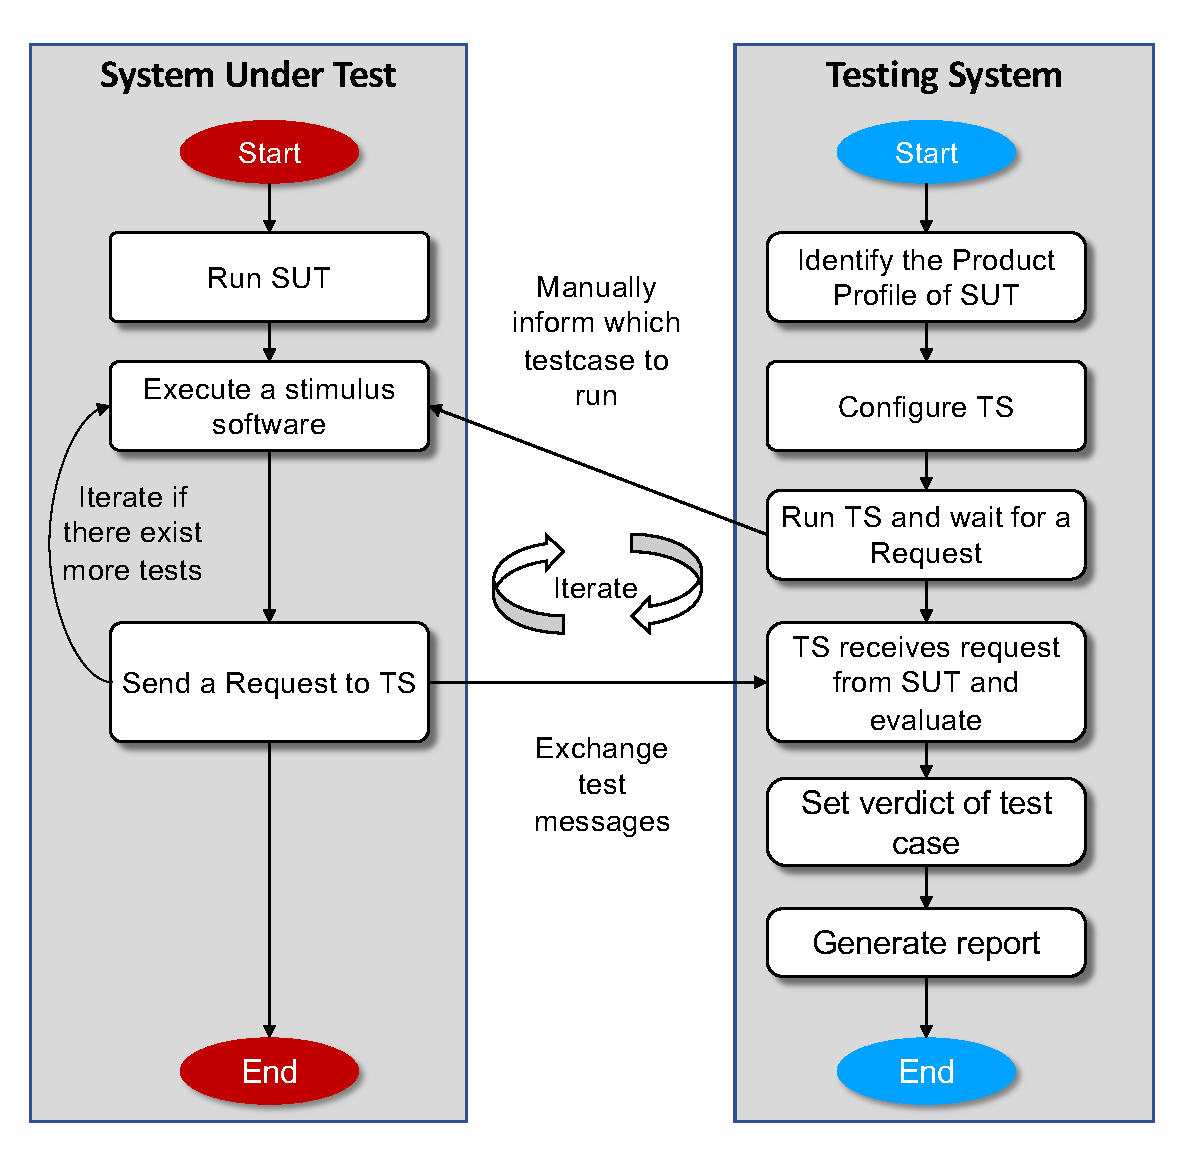
\includegraphics[width=\textwidth]{figures/fig_testing_procedures_in_the_lab.pdf}
    \caption{Flow chart of IoT conformance testing procedures between TS
and constraint SUT that needs external stimulus software.}
    \label{fig:testing_procedures_in_lab}
\end{figure}
In parallel, while the test case is running in the TS and waiting for a specific request from SUT, one of operations such as create, read, update, or delete is constructed with headers and body format, and sent to the TS. As soon as the TS receives the request from the SUT, the TS completes the execution of the test case. Lastly, the TS sets the verdict of the test case as a result, and there are four types of verdicts: Pass-SUT behaves correctly according to the test purpose, Fail-SUT violates its test purpose, Inconclusive-neither a pass nor a fail can be assigned, Error-errors in the testing system~\cite{muhammad2008introduction}. After finishing all testing procedures, if the SUT has more features to test, the tester selects and runs each test case in the testing loop again. When the execution of all test cases is completed, the TS generates an overall report. Based on the report, if successful, this tested IoT device gets a certificate as a correct implementation of the standard.

As indicated in the flow chart of Fig.~\ref{fig:testing_procedures_in_lab}, some steps are executed in iterative manner. These steps in the testing procedures require human intervention for manual execution. The tester needs to select and run the test case in the TS and generate a specific request from the SUT according to the test cases. Performing these steps in a loop manually is a hectic and time consuming job, and it leads to inevitable mistakes and errors in the test report~\cite{gonccalves2017influence}. In this regard, assuming a situation where a tester wants to test an IoT device against four test cases which are named Test Case-1 (TC-1), TC-2, TC-3, and TC-4. The tester run the TC-1 in the TS, and the TS waits for the request from the SUT. Then, the tester initiates a request from the SUT according to the TC-1. The TS receives the request and completes the execution of the TC-1 and sets the verdict. As assumed, the tester needs to run all four test cases to successfully perform the conformance testing. As a next step, the tester runs the TC-2 in the TS, but mistakenly initiates the wrong request from the SUT. The request from the SUT is not in accordance with the TC-2 expectation, and it triggers a false request. The overall report is then erroneous and affects the outcome of the certification process. This typical conformance testing method of IoT applications is not well capable for the IoT applications. There are many SMEs and individual developers that produce large amount of IoT applications. Therefore, it is legitimate to consider and examine the automatic conformance testing in the field of IoT. The key to the automatic conformance testing procedure for the IoT applications is to initiate and handle the trigger messages between the TS and the SUT to exchange information. In the next section, we thoroughly explain the triggering methodology along with the additional testing components and show how to turn exciting conformance testing approach into automated conformance testing.


\subsubsection{Automated IoT testing architecture and procedures}
In general, for the IoT application testing, after turning on the testing system, a testing expert may directly execute a test case and manually pass a specific requested message to the testing system to determine whether it is suitable. However, the problem is that testing experts have to manually run around dozens or hundreds test cases on IoT application functions, and during the testing process, testing experts might get unexpected testing errors, for example due to sending unintended information to testing system. Therefore, automated IoT testing architecture including Triggering message and Upper Tester (UT) was developed to support the automated conformance testing without human intervention. Figure.~\ref{fig:architecture_of_automatic_conf_testing} shows the architecture for automatic conformance testing of the IoT applications in a testing lab.

\begin{figure}[H]
	\centering
	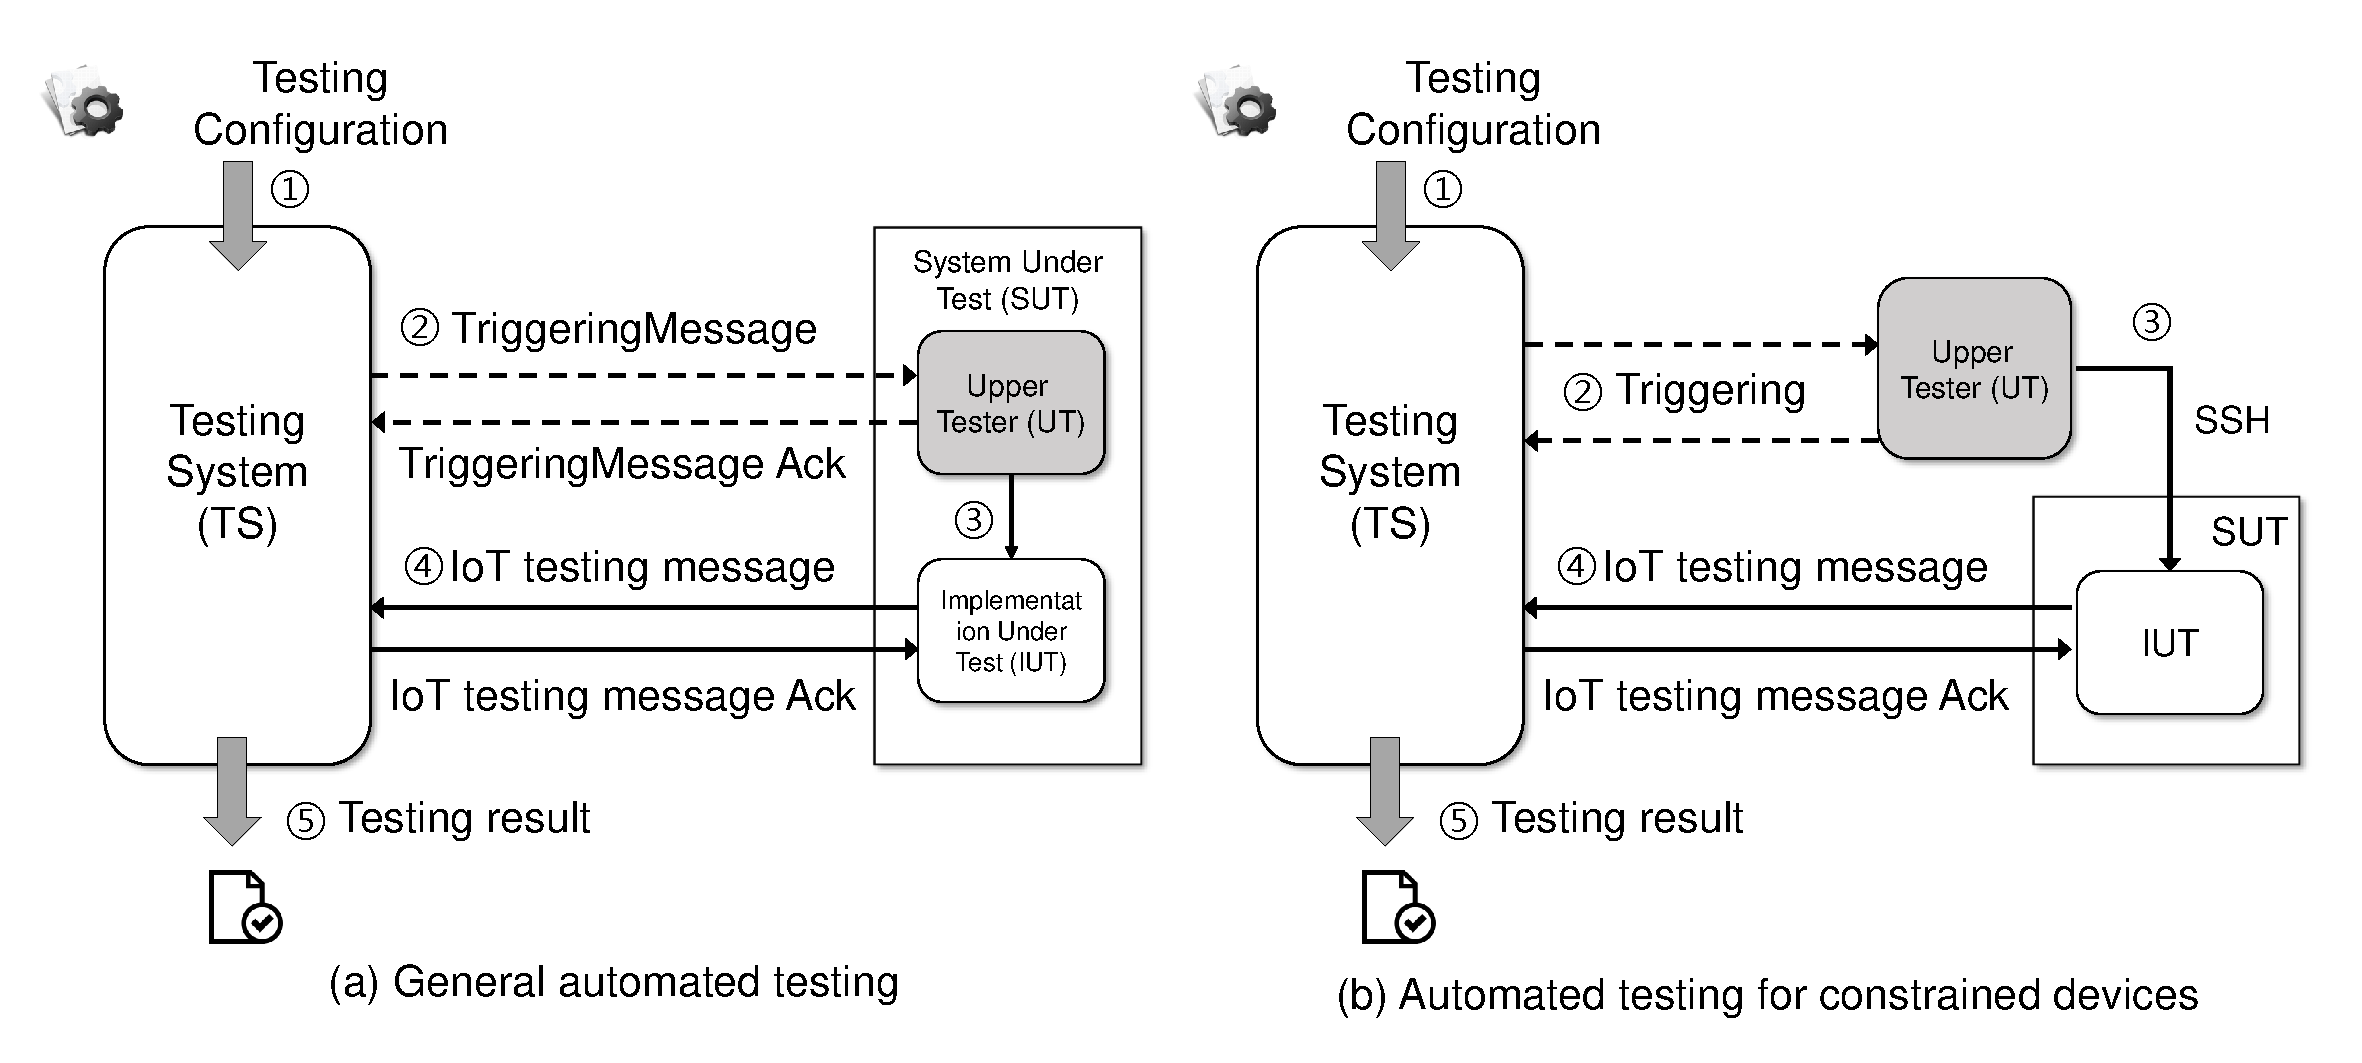
\includegraphics[height=8cm, width=\textwidth]{figures/fig_automated_testing_architecture.pdf}
    \caption{The architecture of automatic conformance testing}
    \label{fig:architecture_of_automatic_conf_testing}
\end{figure}

\begin{itemize}
    \item Testing Configuration: is the testing configuration files that contain the testing parameters written by the testing experts about what testing to perform. The testing parameters to perform specific testing cases can be IP address of testing system, test case name, IoT protocols, serialization formats and so on.
    
    \item Triggering message: is standardised message between the TS and the Upper Tester (UT). In order for TS to perform particular tests, it has to deliver the information based on the testing configuration. That is, the TS parses the configuration file and makes the triggering message including testing case name, protocol, serialization information coming from configuration file. As a next step, the TS delivers triggering message to the UT to start the conformance testing.
    
    \item Upper Tester (UT): is the key testing component that performs the triggering mechanism and reduces human intervention by automating the conformance testing process of the IoT applications. The UT receives the triggering message from the TS, and commands to the Implementation Under Test (IUT) that is a protocol implementation considered as an actual object performing communications. Triggering messages are standardized and to be sent between the TS and the UT. However, the way of performing the specific functions of the IUT can be implemented according to the IoT application manufacturers’ development policies. 
\end{itemize}

The actual procedures of the automatic conformance testing is similar to the procedures shown in the flow chart in Fig.~\ref{fig:testing_procedures_in_lab}, but in this subsection, the more detail procedures of automated conformance testing are provided. By using the two functionalities defined above, automated conformance testing for IoT applications can be performed and the general automated testing procedures are as described Fig.~\ref{fig:architecture_of_automatic_conf_testing}. (a).

\begin{enumerate}
    \item [1)] The testing expert writes about what testing to perform on Testing Configuration and executes a testing case for a IoT device to be tested.
    \item [2)] The testing system then delivers a triggering message containing the testing information to the UT. The triggering message contains the test case name, serialization, IoT protocol type, the address and port information of the TS. Also, if the testing system executes the test cases regarding the POST or PUT method, information about what device data should be sent to the TS is included.
    \item [3)]The UT receiving the triggering message analyzes the message and checks what testing should be performed. The UT then performs a specific function of the IUT, and it delivers the IoT testing message to the TS.
    \item [4-5)] Finally, when the TS receive the IoT testing message, it analyse and verify the message. After that, testing experts can check whether the device is well implemented in accordance with the IoT standard.
\end{enumerate}

\begin{figure}[H]			% Add figure one
	\centering
	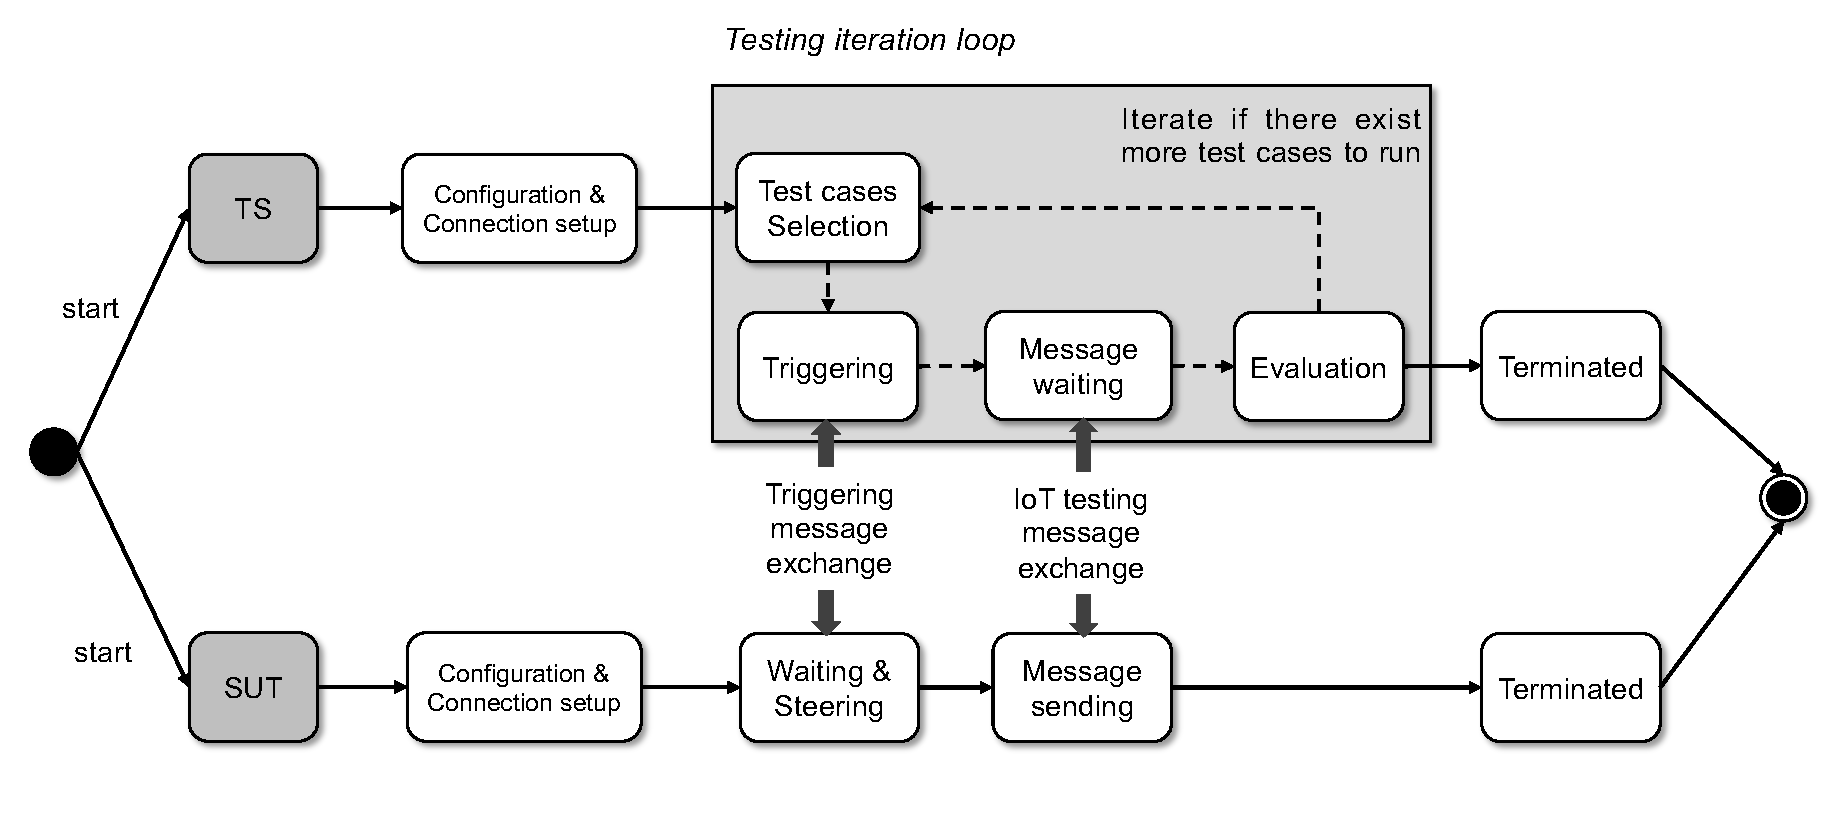
\includegraphics[width=\textwidth]{figures/fig_automated_testing_fsm.pdf}
    \caption{Finite state machine showing automatic conformance testing for IoT Application}
    \label{fig:finite_state_machine_for_conf_testing}
\end{figure}

However, these previous procedures are only for the IoT applications having rich computation resources since UT is based on the HTTP server. There are only a few IoT devices can keep running the UT, and resource-constrained IoT devices are not suitable to deal with the UT as an HTTP server. In these resource constrained IoT devices, the UT cannot reside inside the SUT. To address this particular issue of testing, the UT that runs in resource-constrained IoT devices can dwell outside the SUT, which is depicted in Fig.~\ref{fig:architecture_of_automatic_conf_testing} (b). There are various approaches to set up communication between the UT and the IUT, for example, Secure Shell (SSH) or Telnet. Accordingly, by using one of these options, the UT can communicate to the IUT in a similar way and also it can invoke a specific operation to the IUT. For more detailed procedures of automated conformance testing, a finite state machine showing automatic conformance testing for IoT Application is presented as described in Fig.~\ref{fig:finite_state_machine_for_conf_testing}.

Another key to conduct the automatic conformance testing is to define the standard-based triggering message format between the TS and the UT. Triggering message is developed to deliver the control commands between Testing System and Upper Tester application. This command has to encompass testing parameters that are required for testing a specific test case. In addition, the Triggering message considers that most IoT standards are being developed based on the Resource-Oriented Architecture (ROA) which is one of the software architectures using the REpresentational State Transfer (REST) interfaces~\cite{hong2012resource}. Take into account these requirements, the general triggering message is defined as follows.

\begin{figure}[H]			% Add figure one
	\centering
	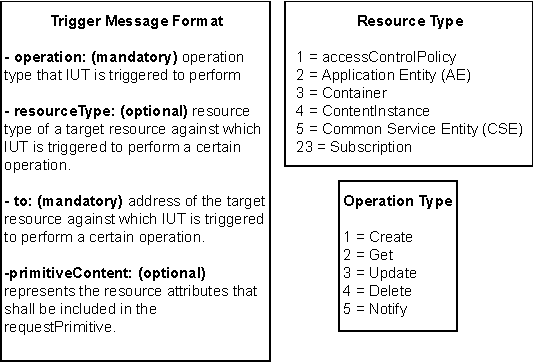
\includegraphics[height=8cm, width=\textwidth]{figures/fig_triggering_message_format.pdf}
    \caption{The Triggering Message Format}
    \label{fig:the_triggering_message_format}
\end{figure}

The body of the request has at most four key/value pairs, such as the operation, ``op" and target testing system, ``to" as mandatory parameters while the resourceType, ``ty" and the primitiveContent, ``pc" are optional parameters. First, ``to" is the IP address of the TS, and it is used when IUT sends the testing request to the TS. The operation ``op" parameter is numerically enumerated on numerous operations that are 1=Create, 2=Get, 3=Update, 4=Delete, and 5=Notify. If the test case has the POST or UPDATE procedure, body information has to be included in the triggering message. resourceType is the virtual representation of all kinds of logical components in the IoT systems such as data instance for saving measured value. primitiveContent represents the resource attributes that shall be included in the specific resource type. Any available information about resource type can be expressed in the form of attributes of the resource type. The response format of the Trigger message is composed with a response code. If the trigger message is correctly formatted by the IUT, then TS sends back the response message that is OK\_REQUEST (2000). Otherwise, it is BAD\_REQUEST (4000). 
\begingroup
\begin{lstlisting}[language=json,firstnumber=1,basicstyle=\ttfamily\footnotesize,backgroundcolor=\color{white},numbersep=1pt, label=lst-trigger, float, caption=Example of TriggerMessage format, label={lst:trigger_format}]
{ 
  "m2m:rqp" :{
    "op": 1, //indicate CREATE operation
    "ty": 2, //indicate AE resource type
    "to": {TEST_SYSTEM_ADDRESS},
    "pc": {"m2m:ae": {
    			"lbl":"UNINITIALIZED" 
    //indicate that attribute labels needs to be included
                	}
          }
      }
}
\end{lstlisting}
\endgroup
The actual payload for the triggering message is shown in Listing.~\ref{lst:trigger_format}. This payload contains the parameter op: 1, which indicates a CREATE operation, ty : 2 indicates the IoT application resource type, the to parameter points to the target resource address in our TS, and pc is an object that contains primitive contents with respect to the oneM2M standard specification. The receiving IoT application uses this pc object while sending the post request to the TS.

By using the approaches, IoT application conformance testing procedures are radically changed. Even though automated testing could seem very trivial, this approach will bring many advantages in terms of reducing testing completion time and errors coming from testers. In this regard, the conformance testing results between manual testing and automated conformance testing to prove the advantages of this approach are explained in the next section.




\subsection{IoT conformance testing performance evaluation}
This subsection shows the experimental results of an automatic conformance testing process for the IoT applications. In addition, oneM2M that is the global IoT standard is used to provide more practical example.

\begin{table}[ht]
\label{ProductProfiles}
\setlength{\tabcolsep}{3pt}

\begin{center}
\begin{tabular}{|p{3cm}|p{9cm}|}
\hline 
\centering Profile & \hspace{3.3cm}Description\\
\hline
\centering  ADN Profile 1 & IoT application sensing data in a constrained IoT
                            device such as a temperature sensor\\
\hline
\centering  ADN Profile 2 & IoT application actuating things in a
                            constrained device such as a dimmed light\\
\hline
\centering  ADN Profile 3 & IoT application in a normal device such as
  a smartphone \\
\hline
\centering  ADN Profile 4 & IoT application in a small originator device \\
\hline
\centering  IN Profile 1 & Server device supporting IoT services\\
\hline
\centering  ASN Profile 1 & IoT application in a normal actuator
                            device \\
\hline
\centering  MN Profile 1 & Gateway devices that support multiple
                           different area network technologies and
                           connect devices\\ 
\hline
\end{tabular}
\end{center}
\caption{oneM2M Product Profiles}
\label{tab:onemwm_adn}
\end{table}

\subsubsection{Evaluation configuration}
As one of the oneM2M activities, oneM2M is developing the testing specification including conformance testing and interoperability testing. According to these specifications, oneM2M test cases based on TTCN-3 is being developed and provided (https://git.onem2m.org/TST/ATS) while oneM2M is defining the oneM2M Product Profiles specification including many feature sets that have to be certified against the testing labs [49]. In this regard, Table~\ref{tab:onemwm_adn} is presented as oneM2M product profiles example.

The oneM2M ADN Profile of Table~\ref{tab:onemwm_adn} to examine the proposed technique was selected. In addition, the evaluation results of conformance testing are generated by using an IoT conformance testing system called oneM2MTester (https://github.com/IoTKETI/oneM2MTester) which is developed based on open source Eclipse Titan for oneM2M platform developers or testing engineers to test and debug their oneM2M implementations during or after the implementation development. In addition, nCUBE-thyme as SUT based on ADN profile was used. The nCUBE-Thyme is an open source for IoT devices, and it is based on the oneM2M standard (https://github.com/IoTKETI/nCube-Thyme-Nodejs). Meanwhile, oneM2M Testing working group is developing and maintaining the oneM2M test cases base on the TTCN-3, and in this code, the automated testing approach proposed in this dissertation has been reflected. Accordingly, the two types of conformance testing by setting the UT active/deactivate parameter in the configuration file can be selected. As shown in Fig.~\ref{fig:the_onem2m_device_testing_performance}, a performance evaluation to show the feasibility and practicality of the proposed conformance testing mechanism was conducted. Conformance testing for AE was performed on a computer with UBUNTU 16.04 LTS OS, an Intel Core i7-7800X CPU @ 3.50 GHz X2 processor, and 8.0 GB of memory.

\begin{figure}[H]			% Add figure one
	\centering
	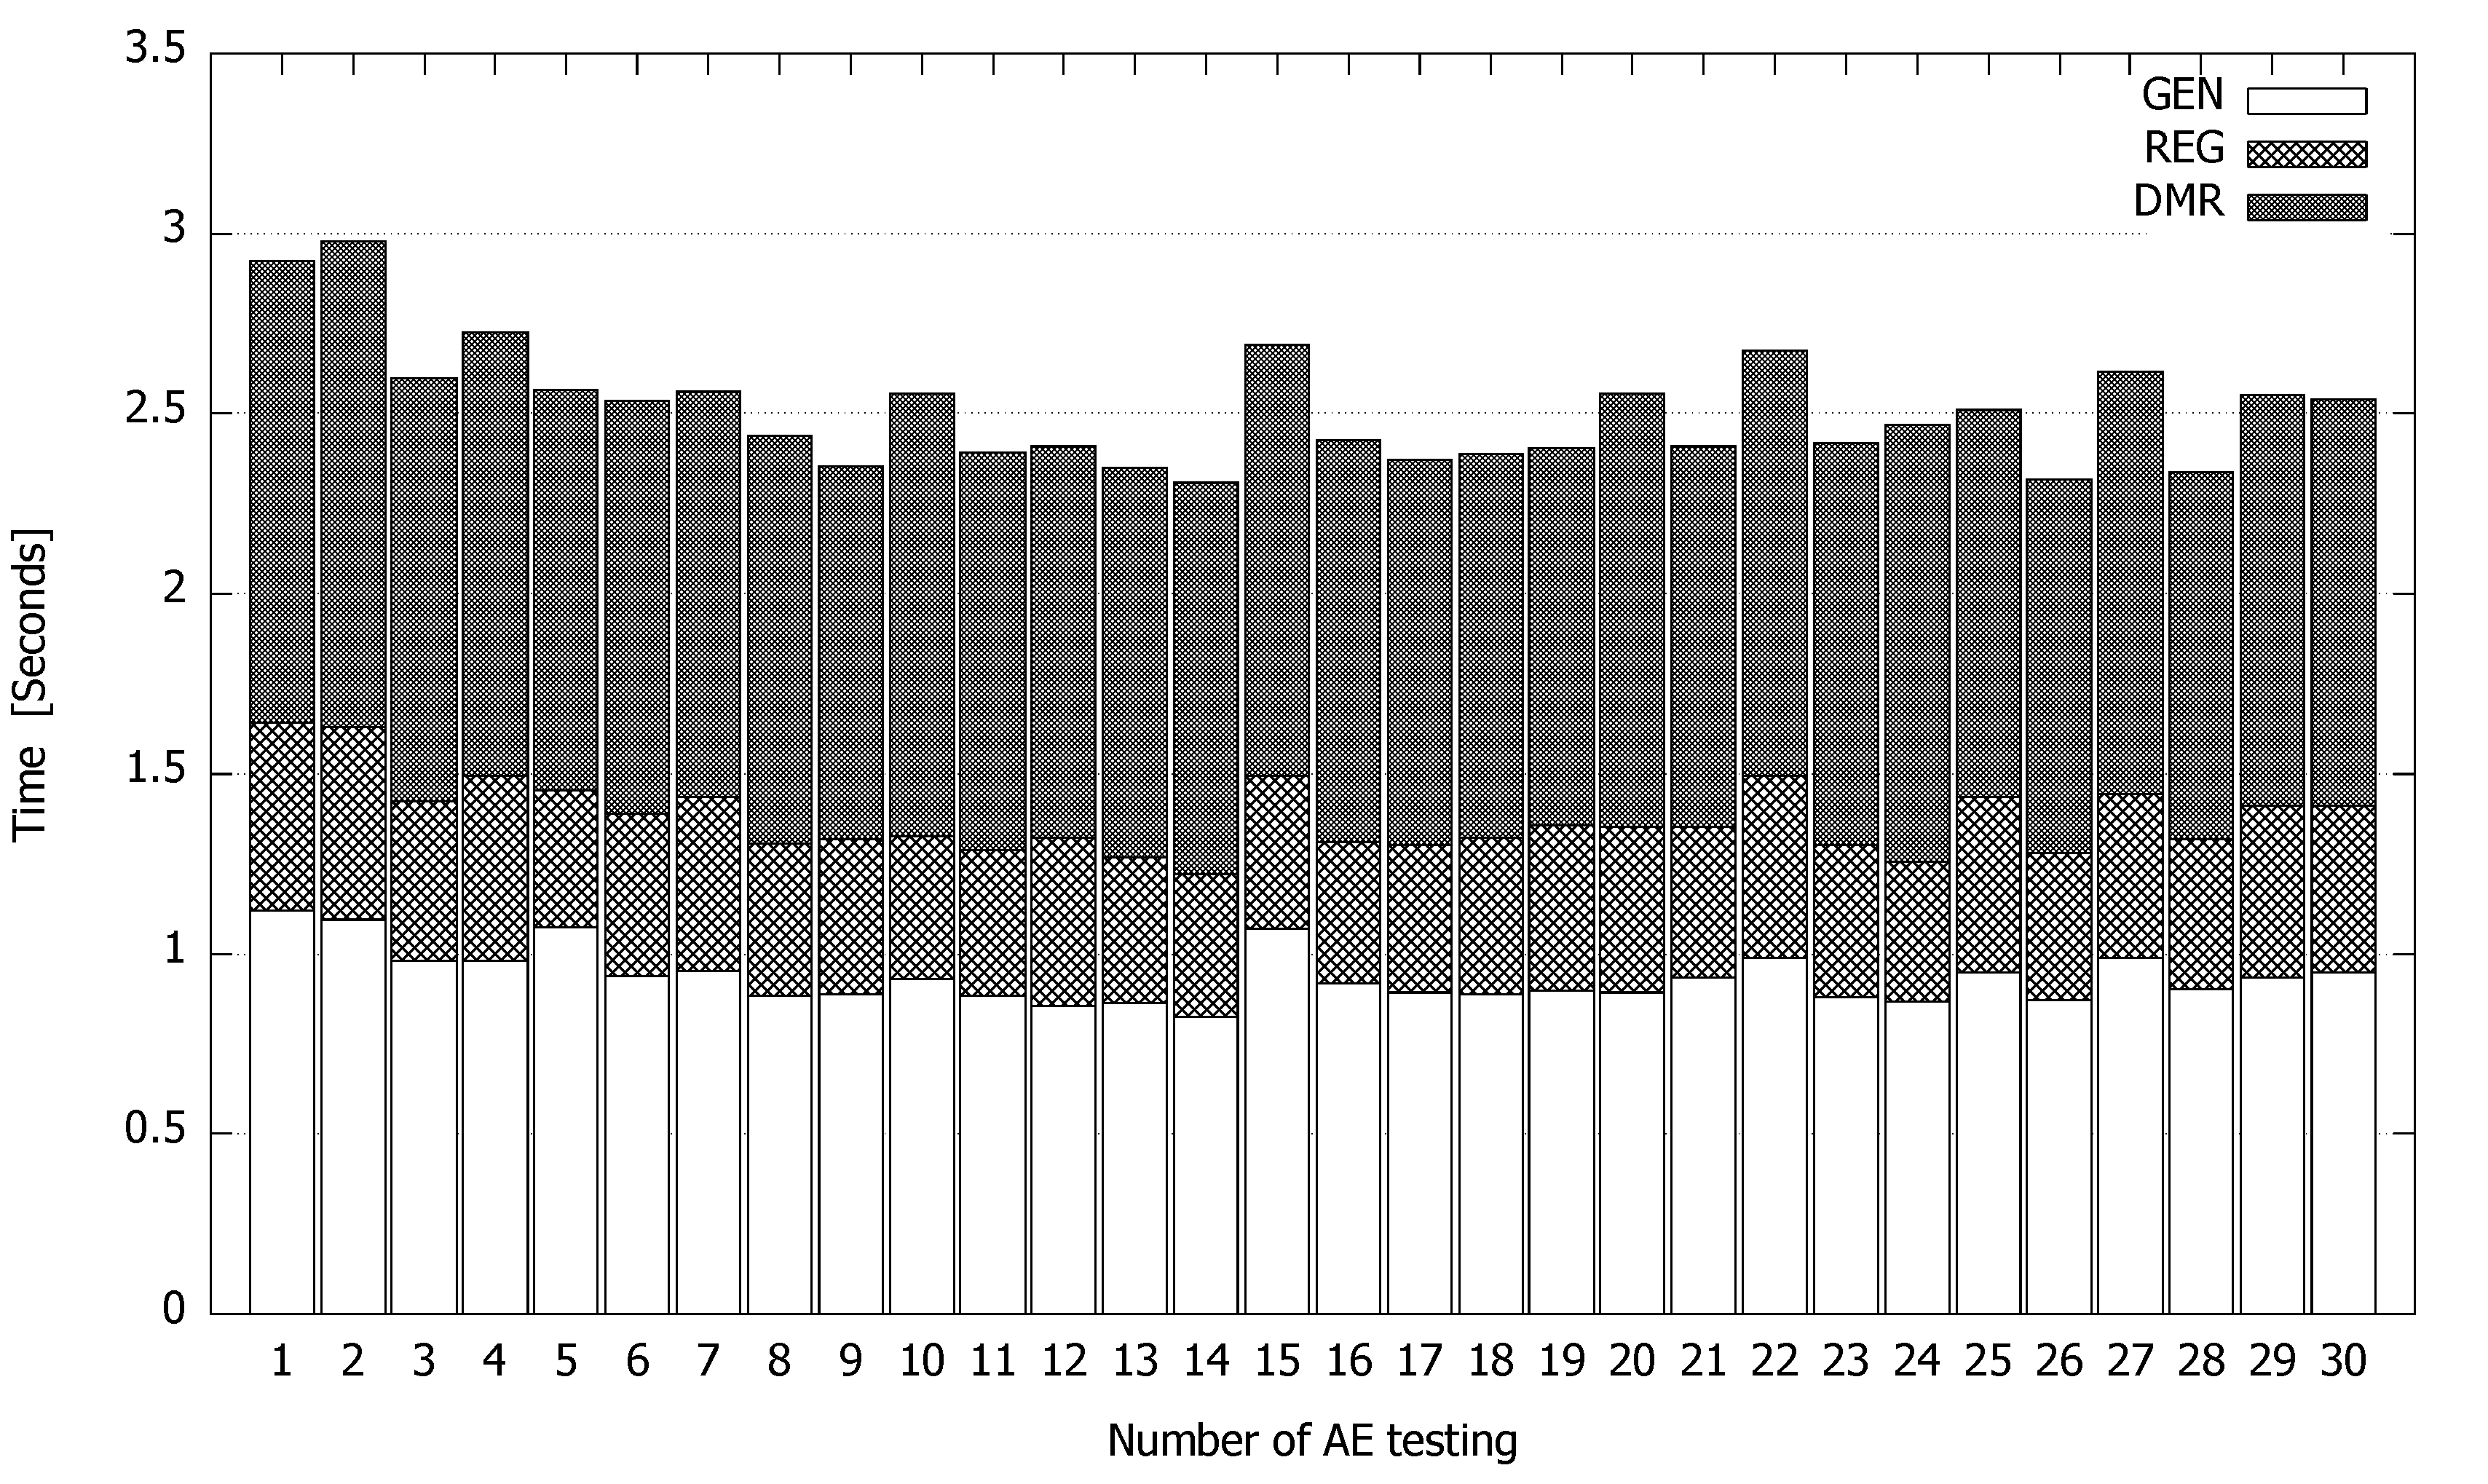
\includegraphics[width=\textwidth]{figures/fig_ae_testing_result.pdf}
    \caption{The oneM2M IoT device testing performance evaluation}
    \label{fig:the_onem2m_device_testing_performance}
\end{figure}


\subsubsection{Testing performance comparison}
For the testing, a total of sixty test cases for general IoT service layer capability (20 test cases), registration of IoT devices (9 test cases), data management-related features (27 test cases), and management of repository functions (4 test cases) were prepared. Such test cases were developed by the oneM2M Test Working Group as sections of testing specifications. An author of this dissertation participated and contributed to the development of the test cases together with other testing experts from industry. For each test case, AE conformance testing was performed 30 times. It took 2.5 seconds to complete one test run for all sixty test cases, and the results showed a standard deviation of 0.165. Figure.~\ref{fig:screen_capture_onem2mtester} shows the GUI of the oneM2MTester after executing a set of test cases.

\begin{table}[ht]
\setlength{\tabcolsep}{3pt}
\begin{center}
\begin{tabular}{|p{1.5cm}|p{2.4cm}|p{1cm}|p{2cm}|p{2cm}|p{2cm}|}
\hline 
\centering Testing Profile & \centering Operation & \centering Items & \centering Automated testing & \centering Hybrid testing & Manual testing \\

\hline
    \centering  \centering GEN & \centering CREATE    & \centering 6 & \centering 0.359 & \centering 11.3 & \hspace{0.4cm} 30.4 \\ 
                               & \centering RETRIEVE  & \centering 6 & \centering 0.306 & \centering 12.7 & \hspace{0.4cm} 27.8 \\ 
                               & \centering UPDATE    & \centering 6 & \centering 0.195 & \centering 9.4 & \hspace{0.4cm} 28.7 \\ 
                               & \centering DELETE    & \centering 6 & \centering 0.261 & \centering 10.5 & \hspace{0.4cm} 29.6 \\
\hline
    \centering  \centering REG & \centering CREATE    & \centering 8 & \centering 0.466 & \centering 14.4 & \hspace{0.4cm} 31.4 \\ 
                               & \centering DELETE    & \centering 1 & \centering 0.205 & \centering 3.5 & \hspace{0.4cm} 30.2 \\
\hline
    \centering  \centering DMR & \centering CREATE    & \centering 13 & \centering 0.782 & \centering 19.7 & \hspace{0.4cm} 54.2 \\ 
                               & \centering RETRIEVE  & \centering 7 & \centering 0.267 & \centering 14.2 & \hspace{0.4cm} 27.8 \\ 
                               & \centering UPDATE    & \centering 4 & \centering 0.117 & \centering 8.8 & \hspace{0.4cm} 21.5 \\ 
                               & \centering DELETE    & \centering 3 & \centering 0.113 & \centering 9.4 & \hspace{0.4cm} 19.6 \\ 

\hline                               
\centering Total & \centering - & \centering 60 & \centering 3.071 (s) & \centering 113.9 (s) & \hspace{0.2cm}274.2 (s) \\
                               
\hline
\end{tabular}
\end{center}
\caption{oneM2M IoT application conformance testing results with three approaches}
\label{tab:testing_comparison}
\end{table}

In order to prove the performance advantage of automated conformance testing, conformance testing for an IoT application with three different testing configurations was conducted, i.e., manual testing, hybrid testing with dedicated stimulus, and automated testing. When the IoT application conformance testing was performed based on the automated testing approach as shown in Table.~\ref{tab:testing_comparison}, it took 3.071 seconds to complete one test set, while stimulus tool-based hybrid testing and manual testing took approximately 113.9 and 274.2 seconds, respectively, to complete one test set.

\begin{figure}[H]			% Add figure one
	\centering
	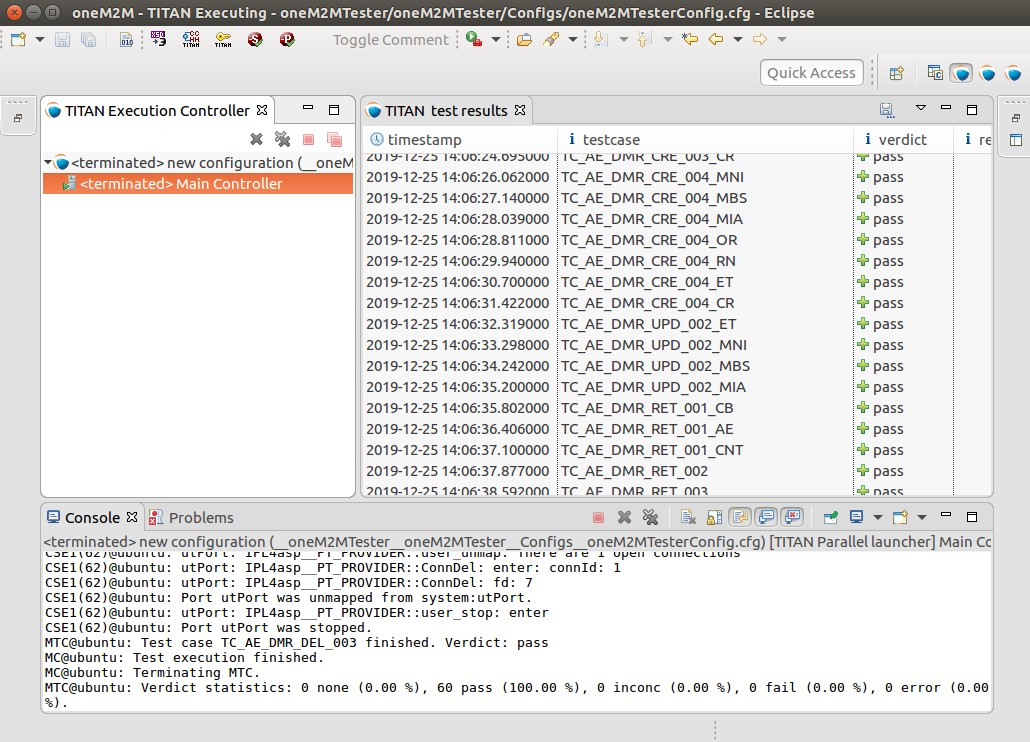
\includegraphics[width=\textwidth]{figures/fig_onem2mtester_testing.jpg}
    \caption{A screen capture of automated conformance testing with oneM2MTester}
    \label{fig:screen_capture_onem2mtester}
\end{figure}

The reason why automated testing performed better than manual and hybrid testing is that all procedures were automated, such as setting the testing parameters and the order of sending and receiving messages between the TS and the SUT so that all test cases could be verified in one execution. In other words, the method using automated testing minimized the tester’s intervention, thereby reducing errors in performing testing. In the case of hybrid testing that uses dedicated software tools with predefined stimulus testers do not need to develop the tools from scratch, and they can reduce the redundant time by using tools’ various support functions such as drop down testing menu, crafting test messages. However, radical problems still remain. To synchronize testing sessions between a testing system and target IoT application, at least two testers have to be involved in. In addition, if a way to test the IoT applications is modified by an organization managing test specifications, these changes have to be reflected as soon as possible; however, it is not an easy task. As described in Table.~\ref{tab:testing_comparison}, by using such tools, testers could get slightly better results than the one from manual testing. However, unless human involvement is fully replaced with standardized triggering message, it is not feasible to test large number of IoT applications.

\subsection{Advanced techniques for IoT standard testing}
There is a high demand for IoT standard testing framework to satisfy cost, coordination, heterogeneity, and scalability requirements. Therefore, to design and propose a novel IoT standard testing framework for resolving the issues, three IoT standard testing related ongoing research is analyzed as a preliminary step. First, F-Interop that uses the remote and distributed approach for conducting the conformance and interoperability testing is illustrated (https://www.f-interop.eu/). As subsequent research, oneM2MTester that aims to develop and distribute an open source oneM2M conformance testing tool is explained to analyze the extensible protocol support and an automated conformance testing approach (https://github.com/IoTKETI/oneM2MTester). Finally, FIESTA-IoT semantic testing which checks the contents of IoT messages to verify that these are properly annotated according to the semantic information based on referenced standards as described (http://fiesta-iot.eu/).

By using the advanced IoT standard testing techniques introduced in these three research, IoT Testing-as-a-Service (IoT-TaaS) architecture is defined. As a result, the newly proposed IoT-TaaS can complement the testing features used in traditional testing, and also it will be helpful in terms of IoT-specific testing issues

\textbf{Automated conformance testing:} with regard to the conformance testing, it is being challenged by the feature of the variability of communication protocols in use. In this regard, IoT protocol bindings and automated testing can reduce the complexity of handling of such variabilities. As one of the standard activities regarding this, oneM2M that is standard for Machine-to-machine (M2M) and the IoT actively standardizes not only the basic specification including conformance and interoperability testing but also advanced IoT testing approaches such as protocol binding for testing and automated approach for IoT devices~\cite{ts0015}. Herein, oneM2M is used to exemplify the IoT device conformance testing.

With the emerging of various IoT services, a range of communication protocols are being used by IoT devices. For instance, HyperText Transfer Protocol (HTTP) is used for general-purpose message transmission while the Message Queuing Telemetry Transport (MQTT) and the Constrained Application Protocol (CoAP) are defined for light-weight message exchange. The IoT testing framework has to consider supporting various communication protocols and standards~\cite{schieferdecker2017iot}. However, it is not easy tasks for SMEs and developers to construct a testing environment for covering all these different protocols and testing features such as monitoring, reporting, and logging. To test these varied standards or protocols, a conformance testing tool that supporting them is required and oneM2MTester is being developed based on this motivation.As described in Fig.~\ref{fig:ttcn-3_conceptual_testing_framework}, TTCN-3 has the testing system and oneM2MTester is based on this architecture. In this architecture, there is an entity called SA to communicate with the SUT. In general, the TTCN-3 only supports standardized encoding schemes such as Basic Encoding Rules (BERs), Abstract Syntax Notation One (ASN.1) and Packed Encoding Rules (PERs). To support the other protocols such as HTTP, MQTT and CoAP, testers need additional procedures to test IoT platforms and devices. In this regard, the oneM2MTester is developing the oneM2M dedicated SA including communication procedures and protocol binding procedures. In this way, any protocol can be added with the extension of the system adapter functionalities.

Compared to the traditional conformance testing, oneM2M conformance testing had the same issues in terms of testing costs. As traditional testing did, developers and vendors have to be physically the same place such as testing labs to conduct conformance testing. This typical conformance testing is not efficient and suitable for individual developers and small to medium-sized enterprises (SMEs) that are producing a lot of IoT devices in terms of testing costs and testing environment configuration since they have to bring their IoT devices to the lab. In addition, if the testing lab is abroad, the business trip fee will account for a very high percentage. Furthermore, oneM2M has defined hundreds of test cases for conformance testing. However, manually conducting lots of test cases is not feasible and time-consuming and highly labor-intensive. Therefore, it is natural to research and bring in the low-cost IoT testing mechanism.

\begin{figure}[H]			% Add figure one
	\centering
	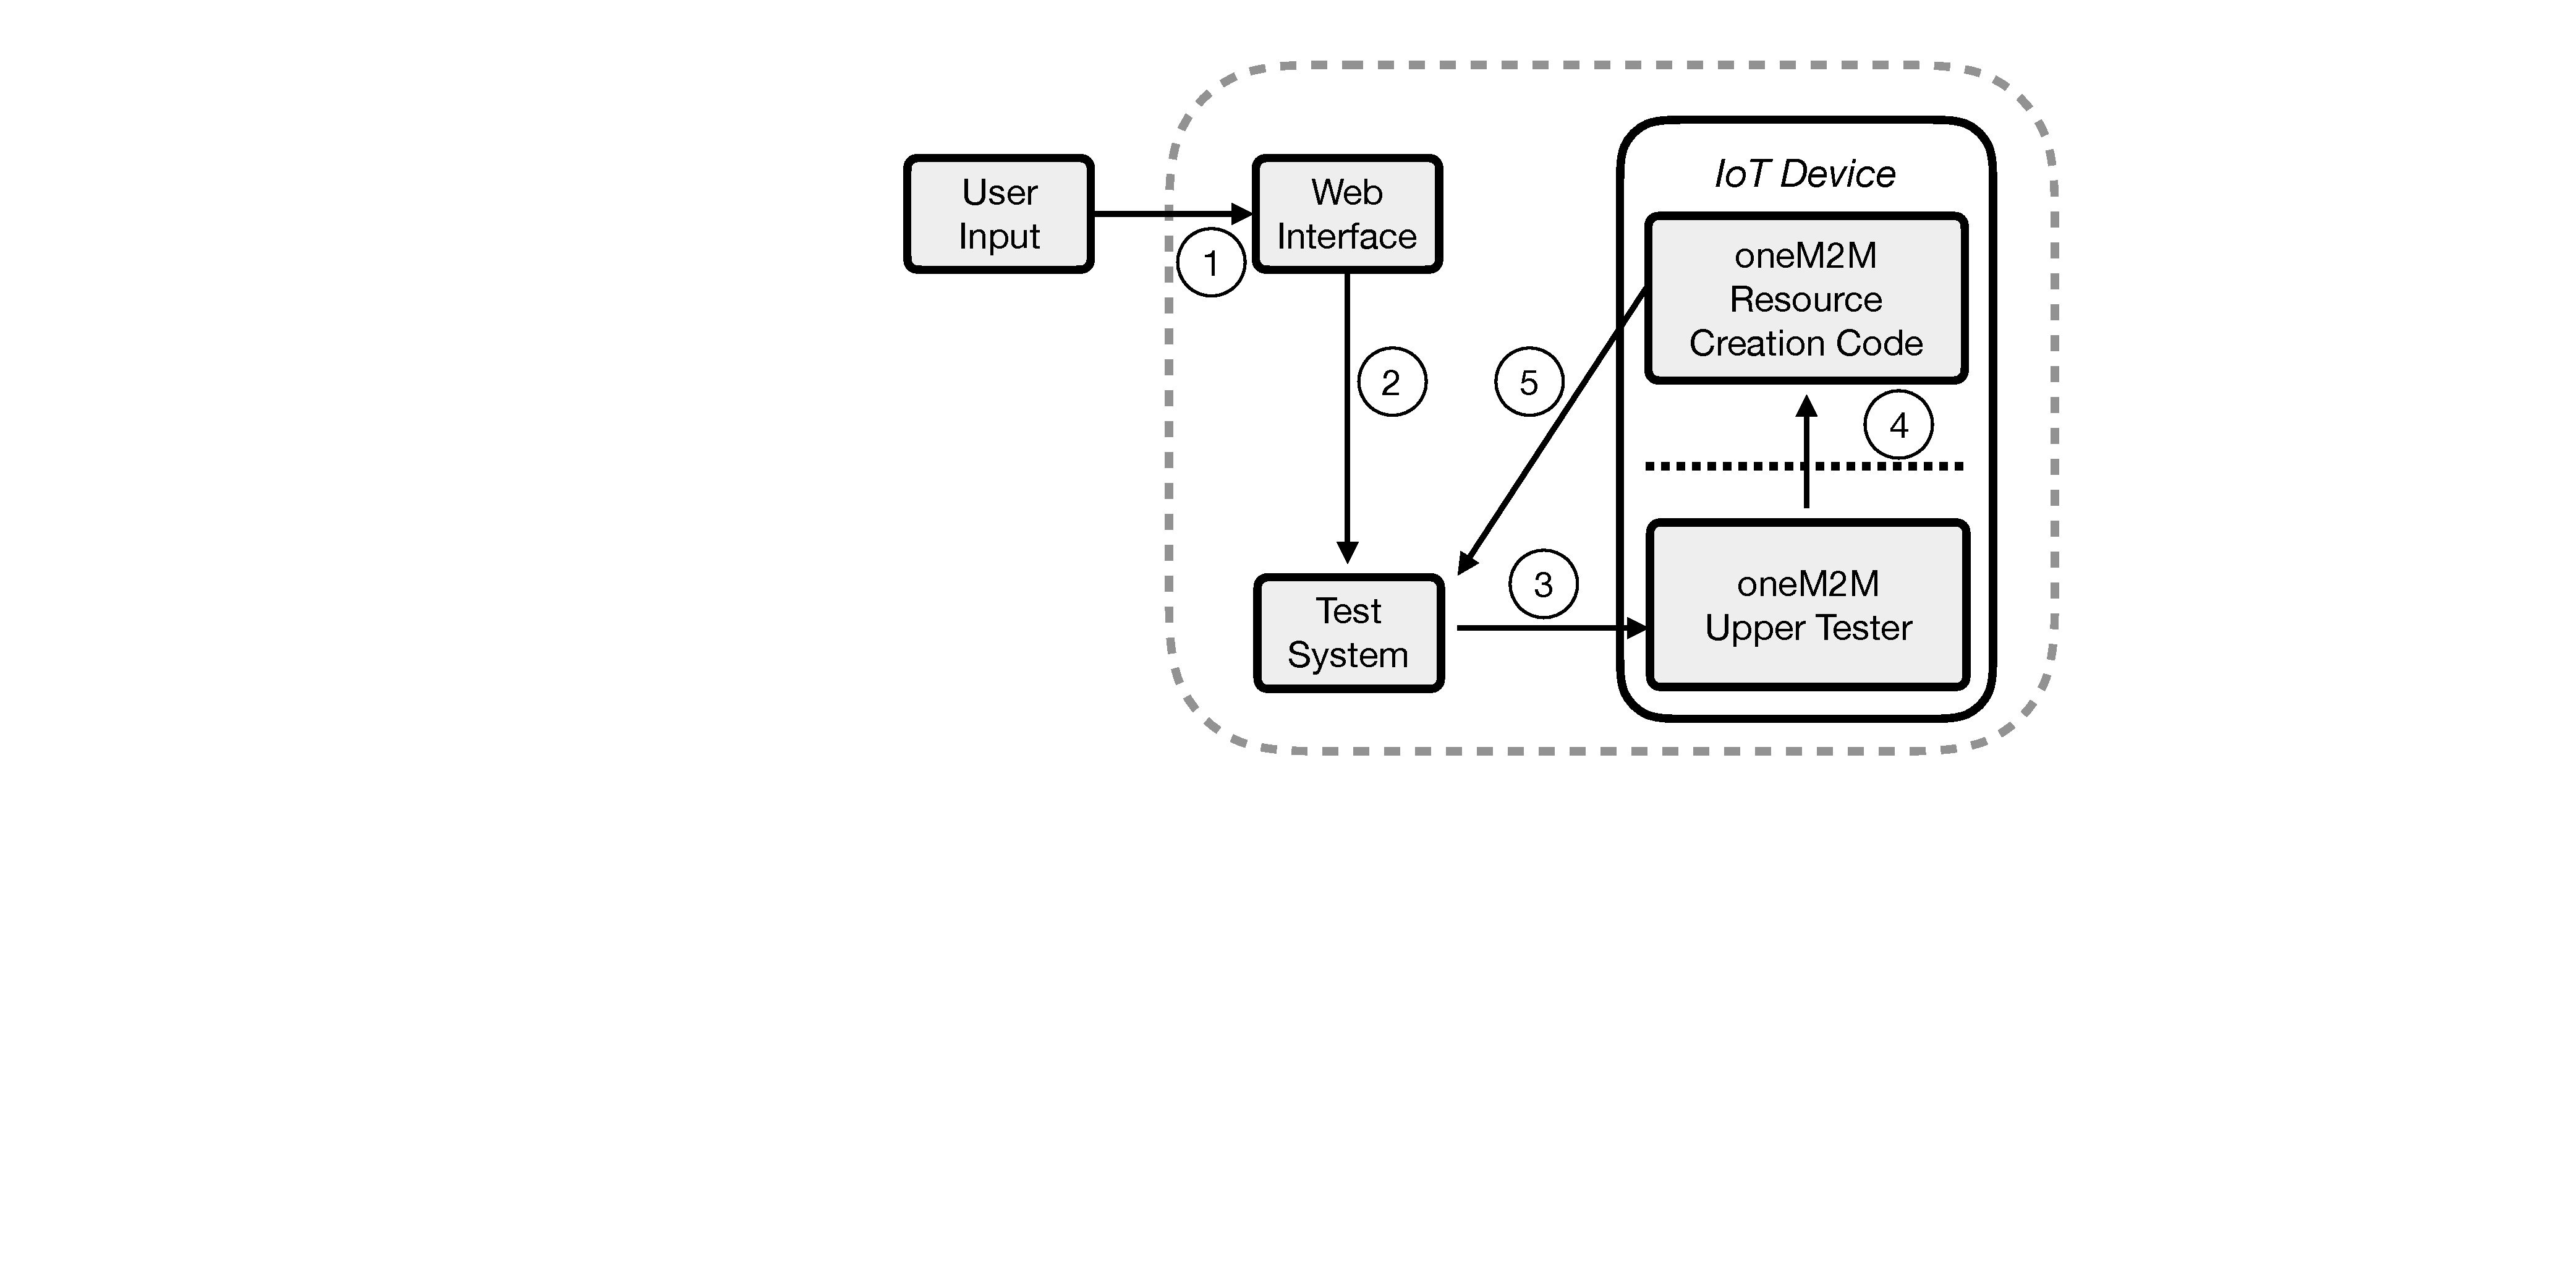
\includegraphics[width=\textwidth]{figures/fig_onem2m-automated-testing-procedure.pdf}
    \caption{Cloud-based automated IoT testing}
    \label{fig:cloud_based_automated_iot_testing}
\end{figure}

Thus, a remote automated conformance testing framework based on web technologies can be considered as a promising solution for resolving the above problems. The core concept of web-based IoT testing is to place core conformance testing components to the cloud and provide the common APIs to the testers for setting the various configuration options based on their testing scenarios. In addition, by allowing other third parties to adopt their own protocol system adapter into the conformance testing system in the cloud, a web-based IoT testing framework can easily adopt new IoT protocols. Regarding the automated conformance testing, the key concept is to trigger the IoT devices to start the communication of a test case. This Upper Tester (UT) is playing the role to realize this. The UT is a logical software component and it can be implemented within an IUT or outside of the IUT according to the capability of the IUT. The upper tester in the SUT is a lightweight server that receives a triggering message from the TS and coordinates the testing behaviour of the SUT. It parses a received triggering message to retrieve the data from the test case in the message body and initiates the predetermined operation. For more practical example of oneM2M automated conformance testing, brief procedures are explained in Fig.~\ref{fig:cloud_based_automated_iot_testing}.

1-2) The testing expert writes about what testing to perform and executes a testing case for a specific IoT device through the web GUI.
3) The testing system then delivers a triggering message containing the testing information to the UT. The triggering message contains the test case name, serialization, protocol type, the address and port information of the testing system. Also, if the testing system executes the test cases regarding the POST or PUT method, Information about what device data should be sent in the body format is included.
4) The UT receiving the triggering message analyzes the message and checks what testing should be performed. The UT then performs a specific function of the IUT and delivers the message to the testing system.
5) Finally, when the device sends responses for the function to be verified in the testing system, verdicts such as pass and fail can be judged, and it can be checked whether the device is well implemented for the standard.

\begin{figure}[H]			% Add figure one
	\centering
	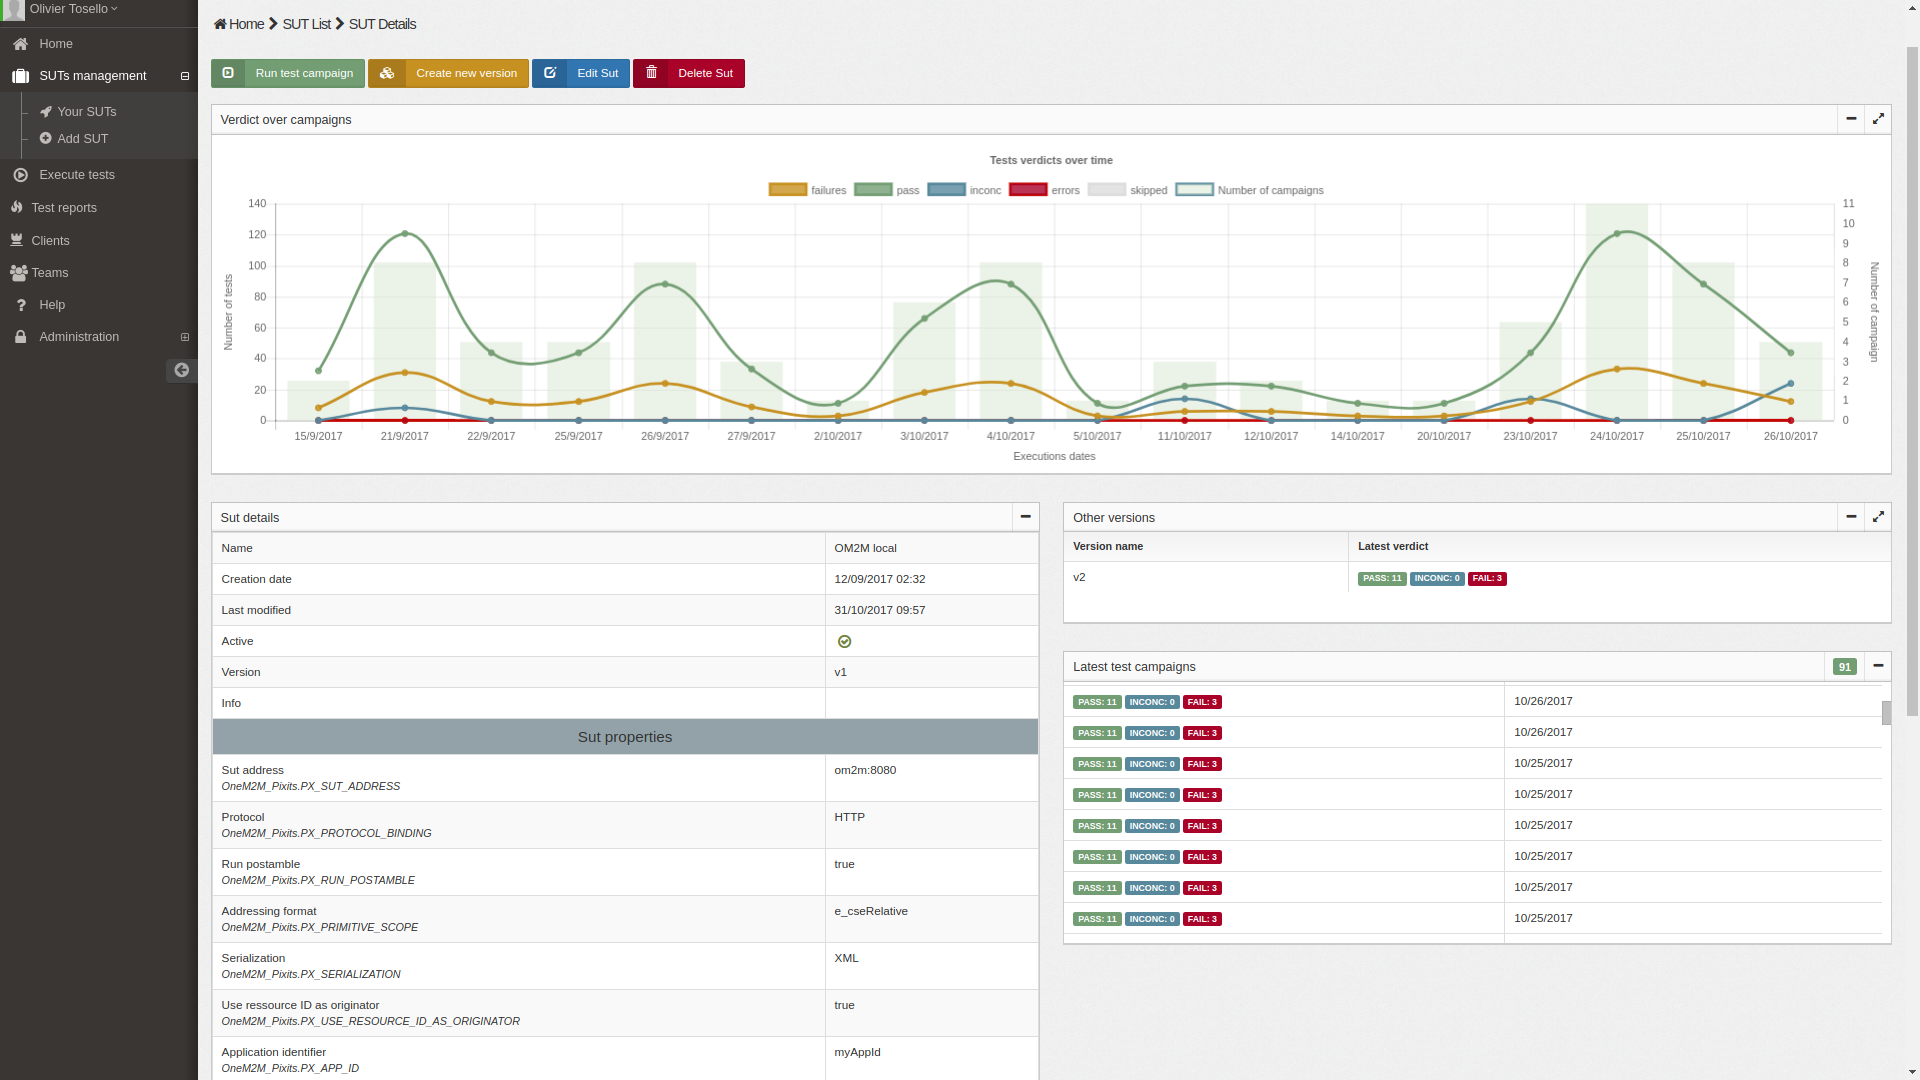
\includegraphics[width=\textwidth]{figures/fig_conftest_web_screen_shot.png}
    \caption{oneM2MTester conformance testing result screen shot capture}
    \label{fig:onem2mtester_conf_testing_screen_capture}
\end{figure}

Based on this concept, oneM2MTester that is web-based oneM2M conformance testing framework is developed. By using this tool, thanks to the remote IoT device testing feature of oneM2MTester, testers can test their IoT devices without visiting IoT testing labs. In addition, with the automated testing approach developers can debug their products during or after the implementation development automatically. Figure.~\ref{fig:onem2mtester_conf_testing_screen_capture} shows the captured screenshot of web-based oneM2MTester, and it shows an overview of the conformance testing results in history against an IUT based on oneM2M.

\textbf{Remote Interoperability testing:}
A testing system for an IoT devices should provide web-based remote testing features. 
The main object of such a testing system is to support a platform for remote testing for accelerating the development speed in terms of standards-based IoT products~\cite{vermesan2014internet}. A testing system called \textit{F-Interop} has the feature that enables the IoT devices testing located in remote places~\cite{ziegler2016f}.

\begin{figure}[H]			% Add figure one
	\centering
	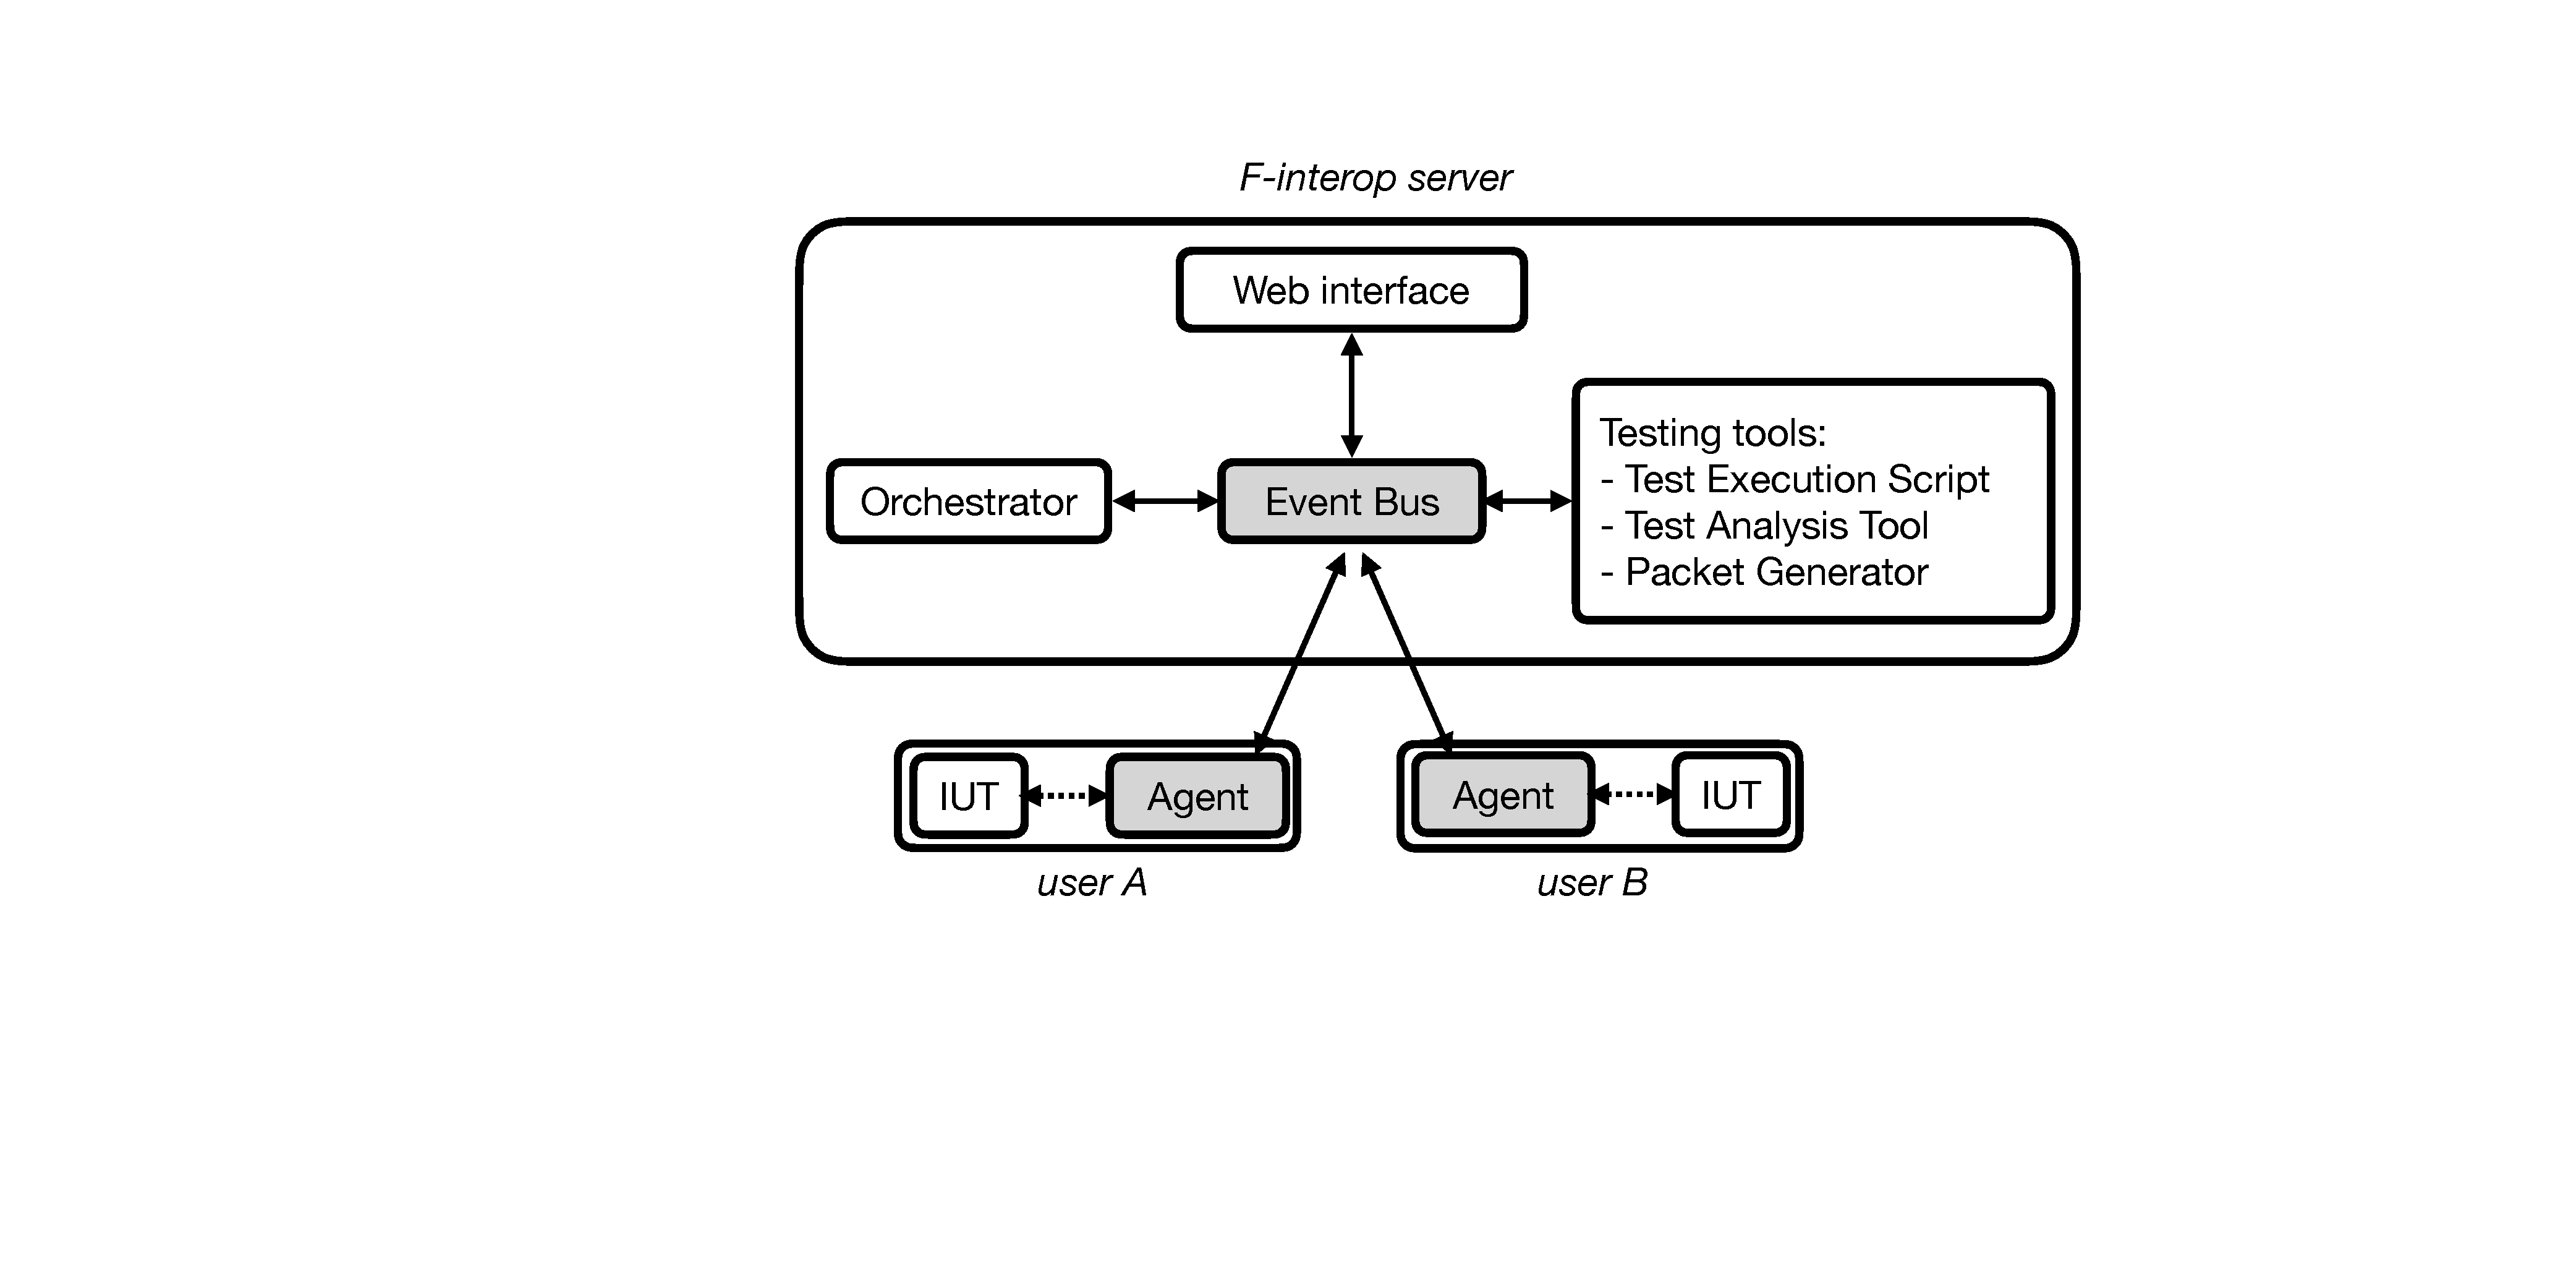
\includegraphics[width=\textwidth]{figures/fig_f-interop-arch.pdf}
    \caption{High-level architecture of F-Interop}
    \label{fig:f_interop_architecture}
\end{figure}

The high-level architecture of F-Interop is depicted in Fig.~\ref{fig:f_interop_architecture}~\cite{leone2016technical}. Compared to traditional software testing, the novelty of F-Interop is using the remote testing approach by having a centralized testing area. For realizing this idea, the testing system provides an agent that is secured communication wrapper for the IUT. After the IUT connection is established through the agent, the testing system creates an isolated area for testing. When the configuration setup is finished, the \textit{test execution script} is executed. This execution consists of three steps. \texttt{STIMULI} to trigger the IUT to initiate a specific action, \texttt{CHECK} to verify communication (e.g. capture the contents of the packet), and \texttt{VERIFY} to reflect the desired result. \textit{Test Analysis Tools} verify output data and behavior after communication. The tool then generates verdicts for the tests in \texttt{PASS}, \texttt{FAIL} and \texttt{INCONCLUSIVE}. The testing system has own packet generator for input generation and supports a web interface to enable testers to check status checking, manually input decision and commands when needed.

\begin{figure}[H]			% Add figure one
	\centering
	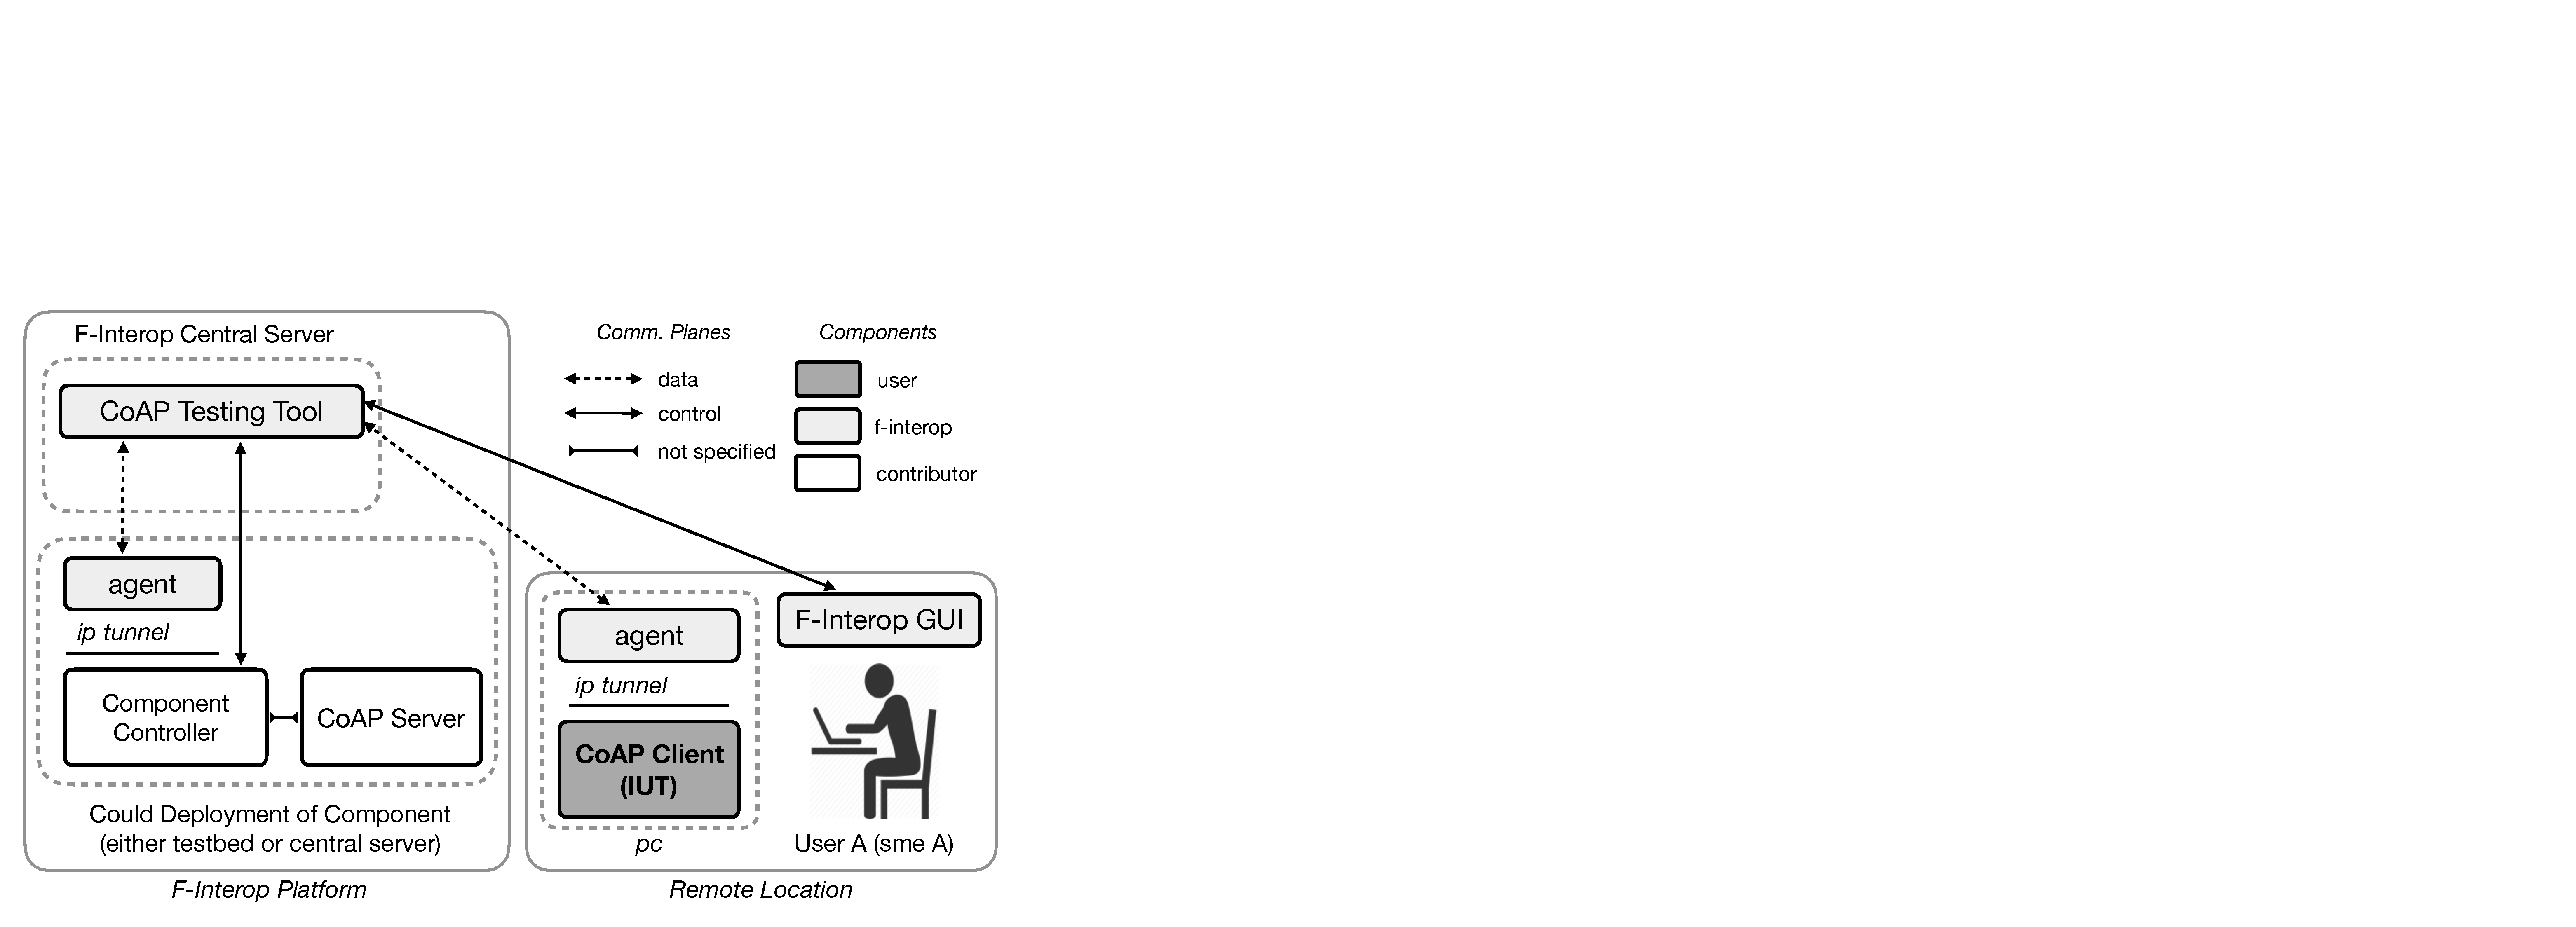
\includegraphics[width=\textwidth]{figures/fig_f-interop-diagram.pdf}
    \caption{Architecture of CoAP protocol testing at F-Interop}
    \label{fig:fi_interop_coap_testing}
\end{figure}

F-Interop's architecture is designed to handle the entire process of IoT interoperability testing with a focus on test management and related tasks such as tracking management and reporting verdicts. All of these tasks are controlled and coordinated by \textit{Orchestrator} that manages the collaboration of various test components such as test sessions, message brokers and access control. Communications are encrypted and managed by the Event Bus. These include control messages, data and log packets being sent to the central event bus implemented in RabbitMQ (https://www.rabbitmq.com/). This centralized communication architecture ensures the independence of each component.

\begin{figure}[H]			% Add figure one
	\centering
	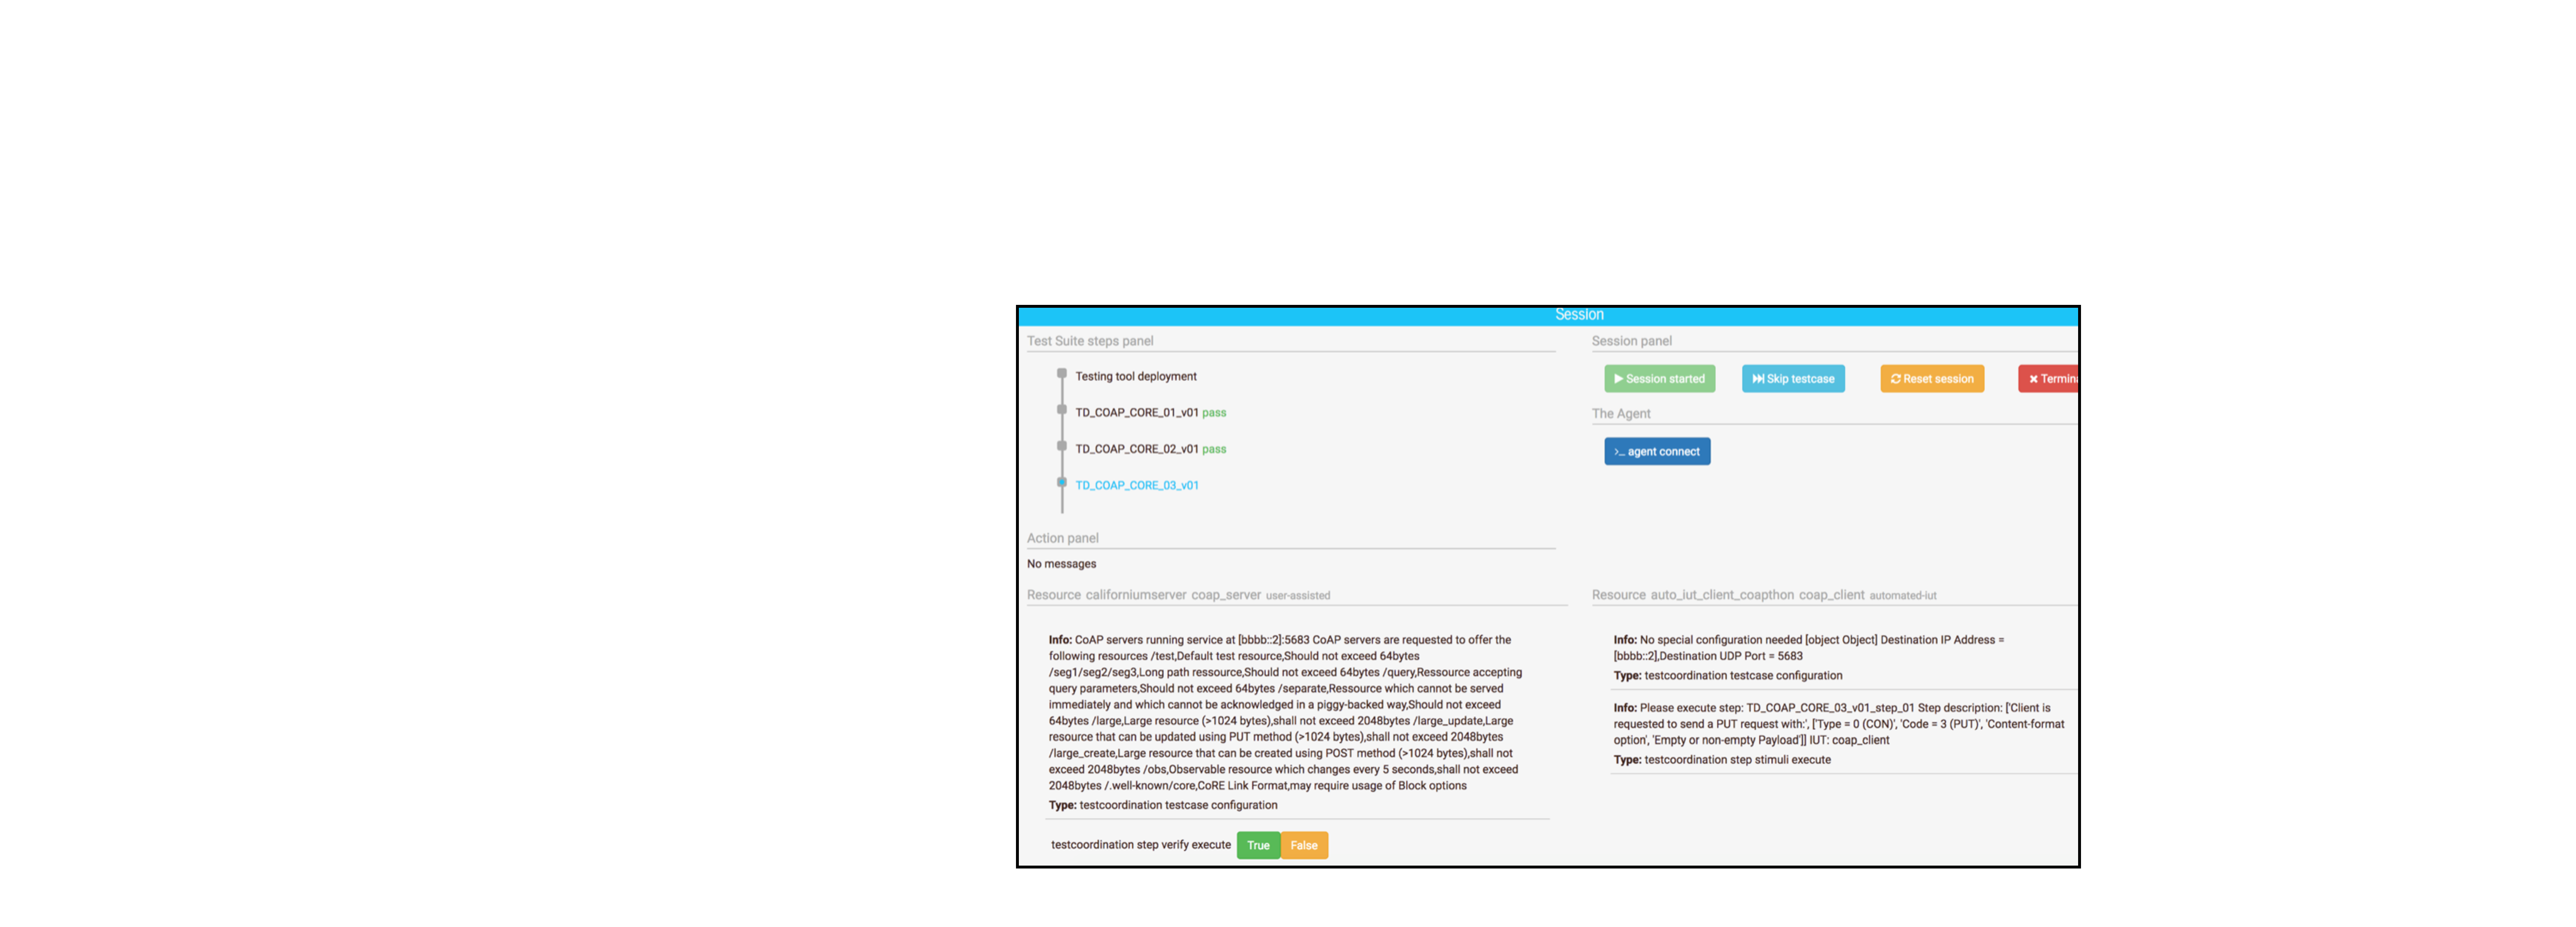
\includegraphics[width=\textwidth]{figures/fig_f-interop-diagram_web.pdf}
    \caption{GUI screen image of CoAP protocol testing as F-Interop}
    \label{fig:f_interop_coap_gui_screen}
\end{figure}

To exemplify the remote interoperability testing, CoAP protocol testing is illustrated. As shown in Fig.~\ref{fig:fi_interop_coap_testing}, F-Interop's CoAP interoperability testing consists of analyzing data exchanged between CoAP IUTs through a CoAP testing tool located on the F-Interop central server. This test tool can support three interoperability scenarios to test CoAP IUTs in remote locations. (1) the IUT is connected to the F-Interop test server. (2) IUT is connected to another CoAP device running in the testbed. (3) The IUT interacts with other vendors' IUTs through the F-Interop testing tool. Using these various test scenarios, the User A can rigorously test the interoperability of the IUT. In addition, the actual F-Interop web GUI is showed in Fig.~\ref{fig:f_interop_coap_gui_screen}.

\textbf{Semantics testing for IoT devices:} In the previous section, protocol-level testing mainly analyzed by researching conformance and interoperability testing. However, IoT platforms and devices are being developed based on different levels. Therefore, it is valuable to test different levels such as semantics.

Semantic testing aims to test the accuracy of the semantic description of an IoT data stream against the standard. Studies conducted on these challenges relating to Semantic Web have concluded that one of the key aspects of achieving semantic interoperability is the ontology and data annotation using these ontologies. Standardization organizations have already defined reference ontology such as ETSI-SAREF ontology (ETSI Smart Appliance Reference ontology), W3C-SSN ontology (Semantic Sensor Network Ontology) and oneM2M basic ontology. Once the reference ontology is defined, one important step for ensuring semantic interoperability is to test its conformance against the reference ontologies. However, Semantic testing of the IoT environment is especially challenging because of the large diversity of semantic modeling methods and a large number of concepts and relations between these concepts. For instance, IoT-Lite optimized performance for handling large and various semantic models of IoT by developing a light-weight semantic model. 

Several research projects are working to address these challenges by proposing and applying these semantic assessment methods and tools. The H2020 \textit{Fiesta-IoT} project is one of the projects that aims to build a unique cloud platform of semantically federated IoT testbeds for new experiments based on semantic technology. The platform provides a unique access point for rich semantic data coming from various types of testbeds (e.g. crowdsensing applications, smart cities, smart campuses and smart buildings). For an appropriate semantic database that provides accurate data about the agreed-upon ontology to be used by experimenters relying on standard semantic technology, semantic verification operations are applied to the incoming data stream. If the data does not meet all the requirements related to syntactic and semantic accuracy, it is rejected to keep the database clean and accurate. Therefore, it provides a full report with a description of all the pitfalls that could lead to modeling errors. It assists ontology developers during the correction process. Semantic testing is essential to achieve semantic interoperability. The case study presented to demonstrate that semantic testing is needed in the IoT industry to verify that IoT systems are working as expected. As we claim, semantic testing should include multiple levels of semantic interpretation, such as vocabulary, syntax, semantics and cardinal accuracy, which are important for semantic interoperability.

One of the main reasons to have a semantic validator is to check for semantic annotations (data annotated for ontology). For example, there is an IoT platform that has introduced a meta-test bed IoT/cloud infrastructure to unite various IoT testbeds distributed around the world. These platforms aim to overcome the barriers between technology and data silos by applying semantic technology. Any user who wants to access data, regardless of location and connected IoT platform, can send data annotated against a common ontology to the semantic repository. From this perspective, the user should check the consistency of the annotation. Otherwise, the platform will reject the data. In this way, the Semantic Validation Tool is a key element of the IoT platform that helps users generate correct annotations. In fact, the tool provides a detailed validation report that lists various errors.

\begin{figure}[H]			% Add figure one
	\centering
	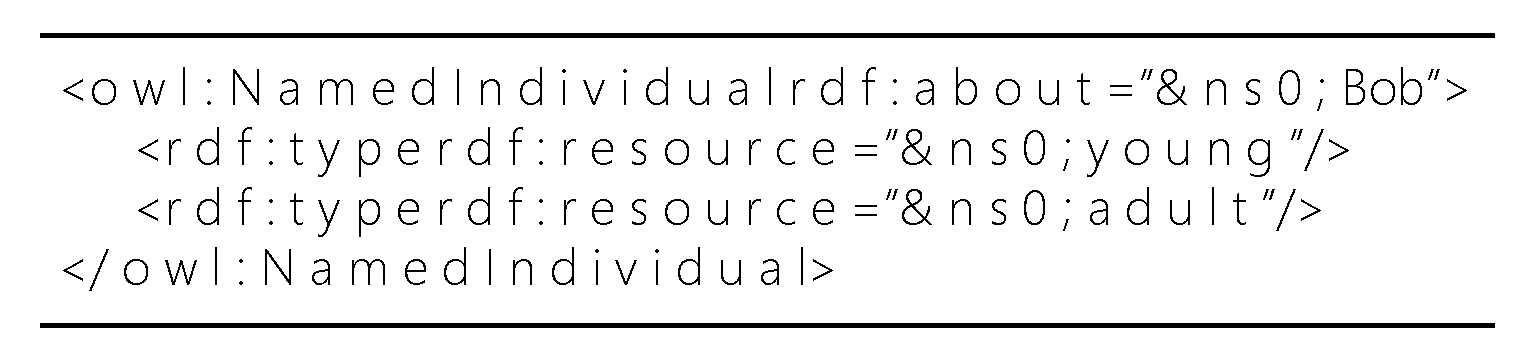
\includegraphics[width=\textwidth]{figures/fig_smantic_validation_example.pdf}
    \caption{Example of invalid semantic resource}
    \label{fig:example_of_invalid_semantic_resource}
\end{figure}

For instance, \textit{Semantic Verification} can be exemplified. Validation tools can determine ontology consistency, identify subsumption relationships among classes, etc. To perform semantic validation, the developers upload the ontology to the tool, then checks the syntactic of ontology format and URI validation and return the reports. The tool also demonstrates the semantic correctness of predicates. For example, consider the list of annotation list in Fig.~\ref{fig:example_of_invalid_semantic_resource}, which contains two classes (adult and young person) defined as common classes. This list includes inconsistencies when defining instances (Bobs) which is the person with young and adult classes. When a developer enters these annotated resources into the validator, the mismatch in annotations results in semantic or logical errors.

\begin{figure}[H]			% Add figure one
	\centering
	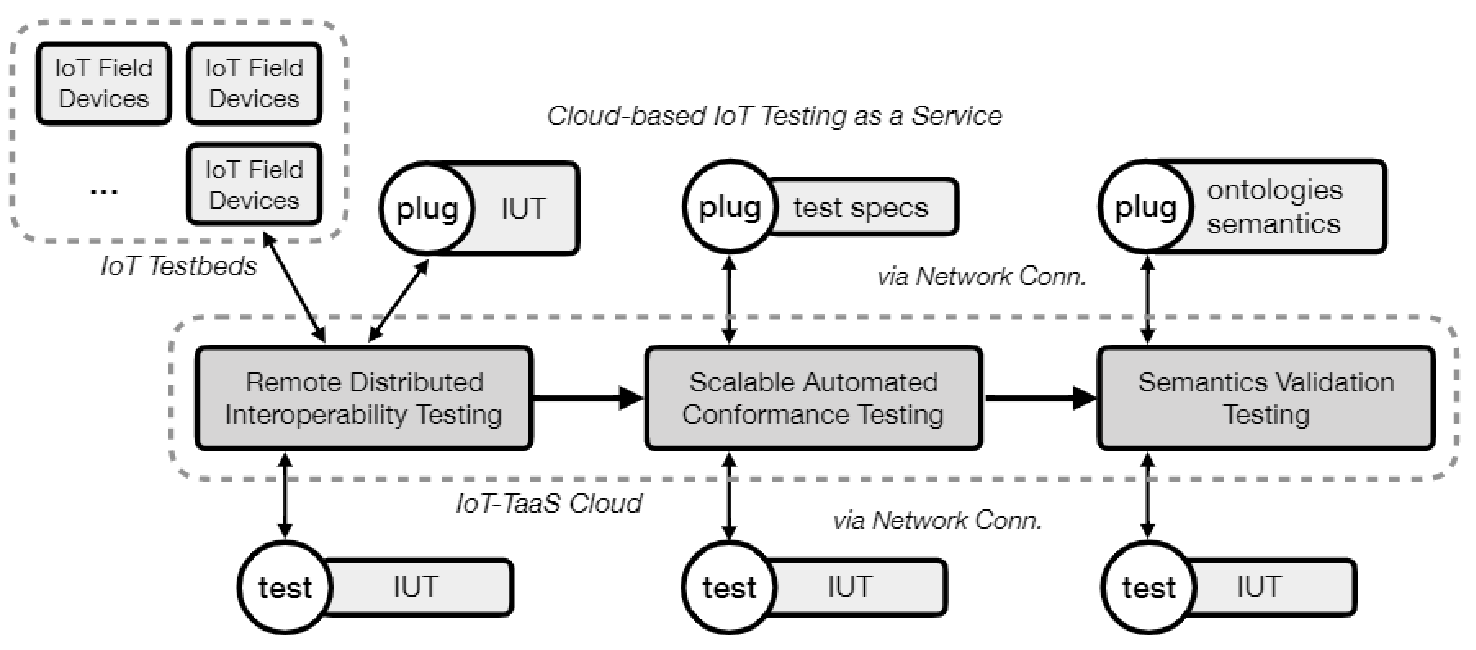
\includegraphics[width=\textwidth]{figures/fig_iot-taas_architecture.pdf}
    \caption{Architecture of cloud-based IoT Testing-as-a-Service}
    \label{fig:iot-taas_architecture}
\end{figure}

This subsection introduced a series of enhancements to the traditional conformance and interoperability testing concepts, along with semantic validation to test various IoT platforms and devices. As these concepts are now implemented and adopted as tools for IoT certifications, it is expected that these concepts will play a key role in the modern IoT testing framework. These three main IoT test concepts can be developed into IoT-TaaS's ``plug and test'' concept as described in Fig.~\ref{fig:iot-taas_architecture}. This plug-and-test concept makes it easy to extend the functionality of the test system without modifying the test system itself. For example, conformance testing can plug test specifications (including test cases and profiles) and perform tests on the IUT. The semantic validation test also enables various ontology depending on the ontology used in the target document and can verify the correctness of the semantics used in the document. Finally, interoperability testing provided by IoT-TaaS allows other field IoT devices to verify the target IoT device. If there is a demand for different types of testing to IoT-TaaS, the new test set cases, ontology information, and new messages can be easily added to the system. These design concepts can provide a practical architectural concept for practitioners designing and implementing IoT-TaaS for the IoT ecosystem. IoT-TaaS offers significant advantages to accelerate the development of standards-based IoT products.

\subsection{Summary}
At present, the IoT combined with technologies such as artificial intelligence and 5G is applied across many industries as well as people’s lives. However, it would be predicted that the operation without proper verification of the IoT applications might cause several problems such as the device or platform not working well, and finally, it makes serious problems to all the industries and people’s lives. Therefore, proper verification must be performed before operating IoT applications. In this regard, the traditional IoT conformance testing method requires testing experts to manually test the IoT applications, and it is not easy to set the testing environment and execute all the test cases manually. Therefore, to solve the problems above, the automated IoT conformance testing approach including architecture and implementation are developed and showed how to conduct automated IoT conformance testing with oneM2M IoT standard. This mechanism has been reflected in the oneM2M IoT standard and being used IoT testing labs such as TTA to test the IoT applications. To conclude, by using the automated testing approach, SMEs will benefit from time and cost, and SDOs can speed up the propagation of the adoption of IoT standards.
\clearpage